%%% The main file. It contains definitions of basic parameters and includes all other parts.

% Meta-data of your thesis (please edit)
\input metadata.tex

% Generate metadata in XMP format for use by the pdfx package
\input xmp.tex

%% Settings for single-side (simplex) printing
% Margins: left 40mm, right 25mm, top and bottom 25mm
% (but beware, LaTeX adds 1in implicitly)
\documentclass[12pt,a4paper]{report}
\setlength\textwidth{145mm}
\setlength\textheight{247mm}
\setlength\oddsidemargin{15mm}
\setlength\evensidemargin{15mm}
\setlength\topmargin{0mm}
\setlength\headsep{0mm}
\setlength\headheight{0mm}
% \openright makes the following text appear on a right-hand page
\let\openright=\clearpage

%% Settings for two-sided (duplex) printing
% \documentclass[12pt,a4paper,twoside,openright]{report}
% \setlength\textwidth{145mm}
% \setlength\textheight{247mm}
% \setlength\oddsidemargin{14.2mm}
% \setlength\evensidemargin{0mm}
% \setlength\topmargin{0mm}
% \setlength\headsep{0mm}
% \setlength\headheight{0mm}
% \let\openright=\cleardoublepage

%% If the thesis has no printed version, symmetric margins look better
% \documentclass[12pt,a4paper]{report}
% \setlength\textwidth{145mm}
% \setlength\textheight{247mm}
% \setlength\oddsidemargin{10mm}
% \setlength\evensidemargin{10mm}
% \setlength\topmargin{0mm}
% \setlength\headsep{0mm}
% \setlength\headheight{0mm}
% \let\openright=\clearpage

%% Generate PDF/A-2u
\usepackage[a-2u]{pdfx}

%% Prefer Latin Modern fonts
\usepackage{lmodern}
% If we are not using LuaTeX, we need to set up character encoding:
\usepackage{iftex}
\ifpdftex
\usepackage[utf8]{inputenc}
\usepackage[T1]{fontenc}
\usepackage{textcomp}
\fi

%% Further useful packages (included in most LaTeX distributions)
\usepackage{amsmath}        % extensions for typesetting of math
\usepackage{amsfonts}       % math fonts
\usepackage{amsthm}         % theorems, definitions, etc.
\usepackage{bm}             % boldface symbols (\bm)
\usepackage{booktabs}       % improved horizontal lines in tables
\usepackage{caption}        % custom captions of floating objects
\usepackage{dcolumn}        % improved alignment of table columns
\usepackage{floatrow}       % custom float environments
\usepackage{graphicx}       % embedding of pictures
\usepackage{indentfirst}    % indent the first paragraph of a chapter
\usepackage[nopatch=item]{microtype}   % micro-typographic refinement
\usepackage{paralist}       % improved enumerate and itemize
\usepackage[nottoc]{tocbibind} % makes sure that bibliography and the lists
			    % of figures/tables are included in the table
			    % of contents
\usepackage{xcolor}         % typesetting in color

\usepackage{multirow}
\usepackage{tabularx} % Required for \bigstrut command
\usepackage{pifont}%
\usepackage{longtable}
\usepackage{ltablex}
\usepackage{acronym}
\usepackage{subcaption}
\usepackage{tikz}



% The hyperref package for clickable links in PDF and also for storing
% metadata to PDF (including the table of contents).
% Most settings are pre-set by the pdfx package.
\hypersetup{unicode}
\hypersetup{breaklinks=true}

% Packages for computer science theses
\usepackage{algpseudocode}  % part of algorithmicx package
\usepackage{algorithm}
\usepackage{fancyvrb}       % improved verbatim environment
\usepackage{listings}       % pretty-printer of source code

% You might want to use cleveref for references
% \usepackage{cleveref}

% Set up formatting of bibliography (references to literature)
% Details can be adjusted in macros.tex.
%
% BEWARE: Different fields of research and different university departments
% have their own customs regarding bibliography. Consult the bibliography
% format with your supervisor.
%
% The basic format according to the ISO 690 standard with numbered references
\usepackage[backend=biber,style=iso-numeric,sorting=none]{biblatex} % style=
% ISO 690 with alphanumeric references (abbreviations of authors' names)
%\usepackage[natbib,style=iso-alphabetic]{biblatex}
% ISO 690 with references Author (year)
%\usepackage[natbib,style=iso-authoryear,backend=biber]{biblatex}


%
% Some fields of research prefer a simple format with numbered references
% (sorting=none tells that bibliography should be listed in citation order)
%\usepackage[natbib,style=numeric,sorting=none]{biblatex}
% Numbered references, but [1,2,3,4,5] is compressed to [1-5]
%\usepackage[natbib,style=numeric-comp,sorting=none]{biblatex}
% A simple format with alphanumeric references:
%\usepackage[natbib,style=alphabetic]{biblatex}

% Load the file with bibliography entries
\addbibresource{bibliography.bib}

% Our definitions of macros (see description inside)
\input macros.tex

%%% Title page and various mandatory informational pages
\begin{document}
%%% Title page of the thesis and other mandatory pages

%%% Inscriptions at the opening page of the hard cover

% We usually do not typeset the hard cover, but if you want to do it, change \iffalse to \iftrue
\iffalse

\pagestyle{empty}
\hypersetup{pageanchor=false}
\begin{center}

\large
Charles University

\medskip

Faculty of Mathematics and Physics

\vfill

{\huge\bf\ThesisTypeTitle}

\vfill

{\huge\bf\ThesisTitle\par}

\vfill
\vfill

\hbox to \hsize{\YearSubmitted\hfil \ThesisAuthor}

\end{center}

\newpage\openright
\setcounter{page}{1}

\fi

%%% Title page of the thesis

\pagestyle{empty}
\hypersetup{pageanchor=false}
\begin{center}

\centerline{\mbox{
\includegraphics[width=166mm]{img/logo-en.pdf}}}

\vspace{-8mm}
\vfill

{\bf\Large\ThesisTypeTitle}

\vfill

{\LARGE\ThesisAuthor}

\vspace{15mm}

{\LARGE\bfseries\ThesisTitle\par}

\vfill

\Department

\vfill

{
\centerline{\vbox{\halign{\hbox to 0.45\hsize{\hfil #}&\hskip 0.5em\parbox[t]{0.45\hsize}{\raggedright #}\cr
Supervisor of the \ThesisTypeName{} thesis:&\Supervisor \cr
\ifx\ThesisType\TypeRig\else
\noalign{\vspace{2mm}}
Study programme:&\StudyProgramme \cr
\fi
}}}}

\vfill

Prague \YearSubmitted

\end{center}

\newpage

%%% A page with a solemn declaration to the thesis

\openright
\hypersetup{pageanchor=true}
\vglue 0pt plus 1fill

\noindent
I declare that I carried out this \ThesisTypeName{} thesis on my own, and only with the cited
sources, literature and other professional sources.
I understand that my work relates to the rights and obligations under the Act No.~121/2000 Sb.,
the Copyright Act, as amended, in particular the fact that the Charles
University has the right to conclude a license agreement on the use of this
work as a school work pursuant to Section 60 subsection 1 of the Copyright~Act.

\vspace{10mm}

\hbox{\hbox to 0.5\hsize{%
In \hbox to 6em{\dotfill} date \hbox to 6em{\dotfill}
\hss}\hbox to 0.5\hsize{\dotfill\quad}}
\smallskip
\hbox{\hbox to 0.5\hsize{}\hbox to 0.5\hsize{\hfil Author's signature\hfil}}

\vspace{20mm}
\newpage

%%% Dedication

\openright

\noindent
\Dedication

\newpage

%%% Mandatory information page of the thesis

\openright
{\InfoPageFont

\vtop to 0.5\vsize{
\setlength\parindent{0mm}
\setlength\parskip{5mm}

Title:
\ThesisTitle

Author:
\ThesisAuthor

\DeptType:
\Department

Supervisor:
\Supervisor, \SupervisorsDepartment

Abstract:
\Abstract

Keywords:
{\def\sep{\unskip, }\ThesisKeywords}

\vfil
}

% In Czech study programmes, it is mandatory to include Czech meta-data:

\ifx\StudyLanguage\LangCS

\vtop to 0.49\vsize{
\setlength\parindent{0mm}
\setlength\parskip{5mm}

Název práce:
\ThesisTitleCS

Autor:
\ThesisAuthor

\DeptTypeCS:
\DepartmentCS

Vedoucí bakalářské práce:
\Supervisor, \SupervisorsDepartmentCS

Abstrakt:
\AbstractCS

Klíčová slova:
{\def\sep{\unskip, }\ThesisKeywordsCS}

\vfil
}

\fi

}

\newpage

%%% Further pages will be numbered, which LaTeX automatically enables at the next chapter start


%%% A page with automatically generated table of contents of the thesis

\tableofcontents


\setlength{\parskip}{10pt} % Set the space between paragraphs to 10pt

%%% Each chapter is kept in a separate file
\chapter*{Introduction}
\addcontentsline{toc}{chapter}{Introduction}


In recent years, the application of artificial intelligence (AI) to traditional board games 
has reached unprecedented heights, showcasing remarkable advancements in strategic gameplay. 
Games such as Go, chess, and poker, each with their unique challenges, have served as testing 
grounds for AI algorithms. Go, known for its large branching factor and complex strategies, 
has been revolutionized by AI, notably with AlphaGo's victories against world champions. 

Sagrada is a dice-drafting board game designed by Adrian Adamescu and Daryl Andrews and published in 2017.
Each player constructs a stained-glass window using dice on a personal rectangular 4×5 board with restrictions 
on the types of dice that can be played on each space. Players gain points by completing public and secret objectives 
for dice placements, and the one with the most points after ten rounds is the winner. In case of a draw in total points
achieved, the tie is broken by other criteria implying that there is always a winner in every game.

Unlike Go and chess, which are deterministic games with no hidden information, Sagrada includes both randomness and hidden information, 
adding layers of complexity to strategic decision-making. Additionally, Sagrada has a high branching factor, 
making its gameplay significantly complex. the motivation behind this study lies in solving the challenges of imperfect information and 
high branching factor in developing a strong AI player for Sagrada.

Prior to the composition of this bachelor's thesis, a digital adaptation of the board game Sagrada had already been released 
by Dire Wolf Digital. There is no public documentation available about the AI players of their implementation.

The primary aim of this study is to evaluate and compare the performance of different AI players in 
my implementation of the digital adaptation of Sagrada. My goal was to implement and analyze various AI strategies, 
including ones such as Minimax, Monte Carlo Tree Search (MCTS), and rules-based agents. This research aims to 
examine the effectiveness of each approach by experimenting with different configurations of the agents.


Through statistical analysis and gameplay simulations, this thesis seeks to provide 
insights into the strengths and weaknesses of AI players, offering valuable implications for the 
development of intelligent gaming agents. 

This thesis will concentrate on the two-player version of the Sagrada board game, although it's designed for 1 to 4 players.
\chapter{Game Description}

In this strategic puzzle game, players compete to create stunning stained glass windows using colorful 
dice and complete different patterns. Each player is tasked with carefully selecting and placing dice to fulfill 
specific pattern requirements while navigating constraints and maximizing their score.

For a comprehensive understanding of the game rules and mechanics, the reader should refer to 
the official rule book provided by the publisher. The rule book  \textcite{Sagradarulesbook} serves as the 
authoritative source for setup instructions, gameplay rules and scoring criteria.

While the official rule book offers a comprehensive overview of Sagrada's gameplay mechanics, it does not 
delve into detailed descriptions of specific components or strategies. In the following sections, I aim 
to fill in the gaps left by the rule book, offering detailed descriptions and strategic insights into 
various aspects of Sagrada's gameplay.



\newcommand{\cmark}{\ding{51}}%
\newcommand{\xmark}{\ding{55}}%

\section{Tool Cards (TC)}
Tool Cards provide unique actions that players can take throughout the game to manipulate dice placements, 
modify their boards, or gain additional benefits. One important attribute of a Tool Card is whether it shifts turns or not.
The ones that don't shift the turn allow the players to make either a passing move or a die-placing move after using the Tool Card.
The following table illustrates the 12 different Tool Cards present in the game marking the ones that shift turns with a \cmark and
the ones that do not shift turns with a \xmark :


\newcolumntype{Y}{>{\hsize=0.6\hsize}X}
\setlength{\extrarowheight}{13pt}

\begin{tabularx}{\textwidth}{>{\bfseries}Y|X}
  Name (Shifts turns) & \textbf{Description} \\ 
  \hline
  1. Copper Foil Furnisher(\xmark) & Allows a player to move a die that is already placed on the board to another position ignoring the shade restriction of the destination space. The player must obey all other placement restrictions. \\  
  2. Eglomise Brush(\xmark) & Allows a player to move a die that is already placed on the board to another position ignoring the color restriction of the destination space. The player must obey all other placement restrictions. \\  
  3. Cork-backed Straightedge(\cmark) & Allows a player to place a die on the board to a space that is not adjacent to any other dice. \\  
  4. Flux Brush(\cmark) & Allows a player to re-roll a die from the Draft Pool. The die must be placed on the board if there is any space where the die could be placed with the re-rolled value. Otherwise, the die is returned to the Draft Pool. \\ 
  5. Flux Remover(\cmark) & Allows a player to choose a die from the Draft Pool, swap it with a random die from the Dice Bag and choose the new die's value. The die must be placed on the board if there is any space where the die could be placed with the re-rolled value. Otherwise, the die is returned to the Draft Pool. \\ 
  6. Glazing Hammer(\xmark) & Allows a player to re-roll all dice in the Draft Pool. This Tool Card may only be used on the second turn of a player before drafting.\\  
  7. Grinding Stone(\cmark) & Allows a player to flip a die from the Draft Pool to its opposite side (6 flips to 1, 5 flips to 2, 4 flips to 3). The player must place the flipped die on the board. The die can be flipped only if it is placeable on the board after the flipping. \\
  8. Grozing Pliers(\cmark) & Allows a player to increase or decrease the value of a die from the Draft Pool by 1. 1 cannot be decreased to 6 and 6 cannot be increased to 1. The player must place the flipped die on the board. The die can be flipped only if it is placeable on the board after the flipping.\\
  9. Lathekin(\xmark) & Allows the player to move exactly two dice that are already placed on the board to other positions obeying all placement restrictions. \\ 
  10. Lens Cutter(\cmark) & Allows a player to swap a die from the Draft Pool with one from the Round Track. After swapping the dice, the new die has to be placed on the board. \\
  11. Running Pliers(\xmark) & Allows a player to immediately draft a die after their first turn. This means that using this Tool Card allows the player to move twice in a row. \\ 
  12. Tap Wheel(\xmark) & Allows a player to move one or two dice of the same color that are already placed on the board to a new position. The color of the dice must match the color of a die on the Round Track. The player must obey all the placement restrictions.
\end{tabularx}

I am using the appellation ``relocating tool cards'' multiple times in the text referring to Tool Cards that allow a player to move one or more dice that are already placed 
on the board to a new position. Namely, these are  \textbf{the Copper Foil Furnisher}, \textbf{the Eglomise Brush}, \textbf{the Tap Wheel} and \textbf{the Lathekin} Tool Cards.


\section{Public Objective Cards (PuOC)}
Public Objective Cards represent shared goals that all players strive to achieve throughout the game. These cards provide additional 
challenges and opportunities for players to earn points based on completing specific patterns. For each completed pattern, the player
receives the satisfaction value that belongs to the Public Objective Card. There are 10 different Public Objective Cards:

\begin{tabularx}{\textwidth}{>{\bfseries}l|X}
  Name & \textbf{Description} \\ 
  \hline
  1. Color Diagonal & Awards one point for each die that has a diagonal neighbor of the same color, regardless of the specific colors involved. \\  
  2. Column Color Variety &  The pattern is fulfilled when a given column contains dice whose colors are all different, ensuring that all spaces within the column are occupied by a die. Completing a pattern is worth 5 points.\\
  3. Column Shade Variety & The pattern is fulfilled when a given column contains dice whose shades are all different, ensuring that all spaces within the column are occupied by a die. Completing a pattern is worth 4 points.\\  
  4. Ligh Shades & Awards two points for every pair of dice with a value of 1 and a value of 2. The position of the dice does not matter.\\ 
  5. Medium Shades & Awards two points for every pair of dice with a value of 3 and a value of 4. The position of the dice does not matter.\\ 
  6. Deep Shades & Awards two points for every pair of dice with a value of 5 and a value of 6. The position of the dice does not matter.\\  
  7. Row Color Variety & The pattern is fulfilled when a given row contains dice of different colors, ensuring that all spaces within the row are occupied by a die. Completing a pattern is worth 6 points.\\
  8. Row Shade Variety & The pattern is fulfilled when a given row contains dice of different shades, ensuring that all spaces within the row are occupied by a die. Completing a pattern is worth 5 points.\\
  9. Color Variety & Awards four points for every set of 1 die of each color. The position of the dice does not matter.\\ 
  10. Shade Variety & Awards four points for every set of 1 die of each shade. The position of the dice does not matter.\\
 \end{tabularx}



\section{Window Pattern Cards (WPC)}

After drafting all the Tool Cards, Public Objective Cards and Private Objective Cards, the game continues with every player choosing a Window
Pattern Card. These cards serve as the basic layout of each player's boards. Every space contains a shade restriction,
a color restriction or no restriction at all. If a space contains a restriction, only dice with matching shades/colors can be placed on it.
To every Window Pattern Card belongs a difficulty number which is given to the player in the form of Favor Tokens. There are the following 
24 Window Pattern Card in the game - the difficulty number is represented by the white circles in the lower right corner of the Window Pattern Cards:

\centerline{\mbox{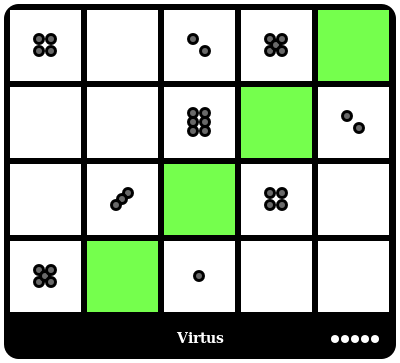
\includegraphics[width=75mm]{img/WPC/Virtus.png}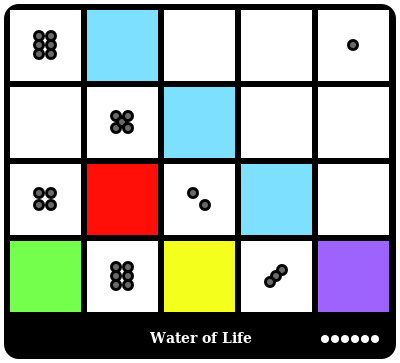
\includegraphics[width=75mm]{img/WPC/WaterofLife.png}}}
\centerline{\mbox{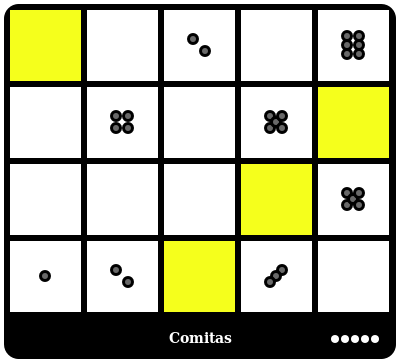
\includegraphics[width=75mm]{img/WPC/Comitas.png}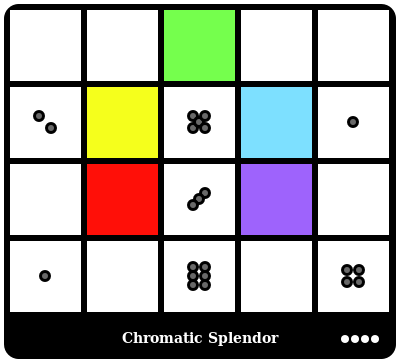
\includegraphics[width=75mm]{img/WPC/ChromaticSplendor.png}}}
\centerline{\mbox{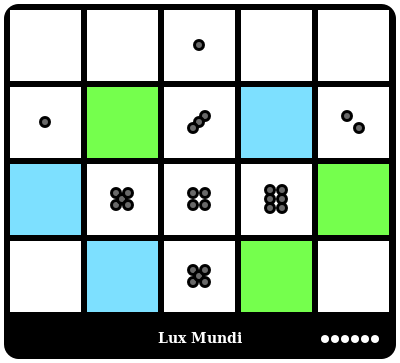
\includegraphics[width=75mm]{img/WPC/LuxMundi.png}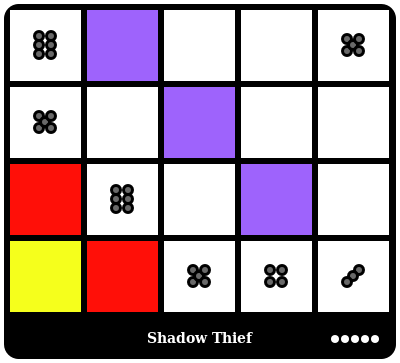
\includegraphics[width=75mm]{img/WPC/ShadowThief.png}}}
\centerline{\mbox{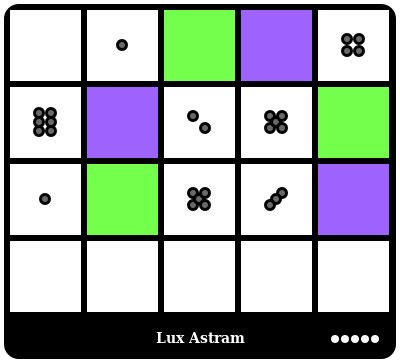
\includegraphics[width=75mm]{img/WPC/LuxAstram.png}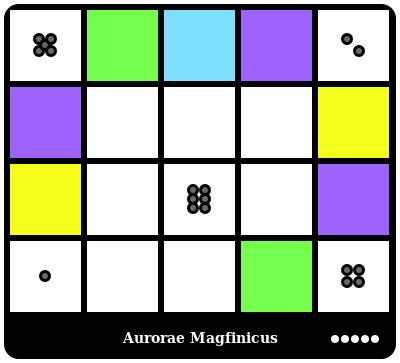
\includegraphics[width=75mm]{img/WPC/AuroraeMagfinicus.png}}}
\centerline{\mbox{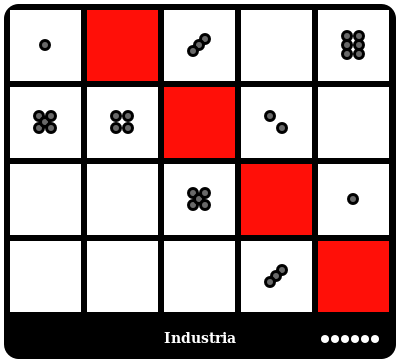
\includegraphics[width=75mm]{img/WPC/Industria.png}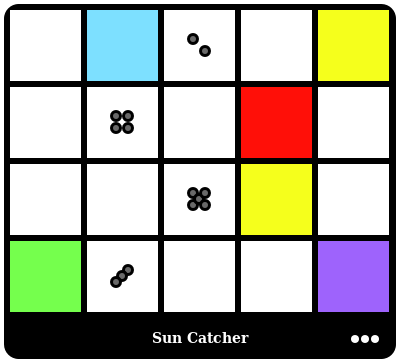
\includegraphics[width=75mm]{img/WPC/SunCatcher.png}}}
\centerline{\mbox{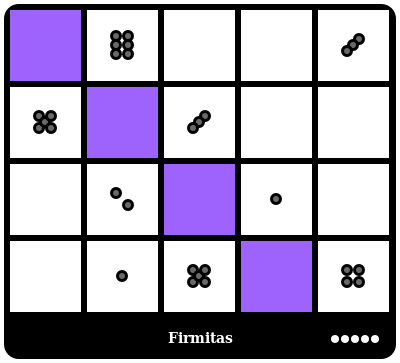
\includegraphics[width=75mm]{img/WPC/Firmitas.png}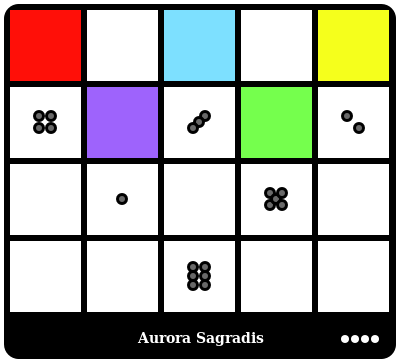
\includegraphics[width=75mm]{img/WPC/AuroraSagradis.png}}}
\centerline{\mbox{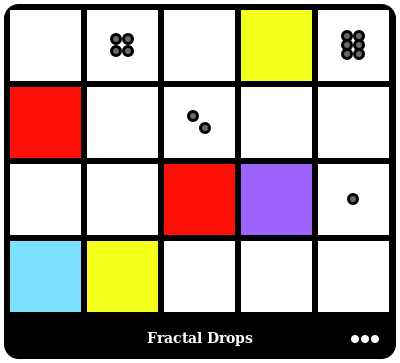
\includegraphics[width=75mm]{img/WPC/FractalDrops.png}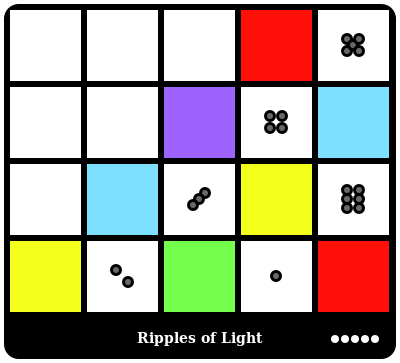
\includegraphics[width=75mm]{img/WPC/RipplesofLight.png}}}
\centerline{\mbox{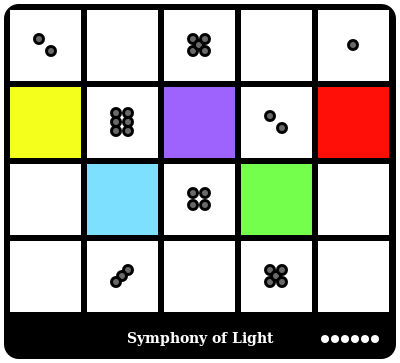
\includegraphics[width=75mm]{img/WPC/SymphonyofLight.png}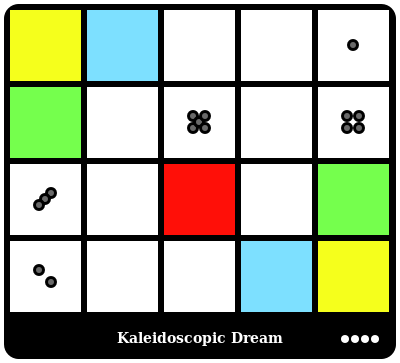
\includegraphics[width=75mm]{img/WPC/KaleidoscopicDream.png}}}
\centerline{\mbox{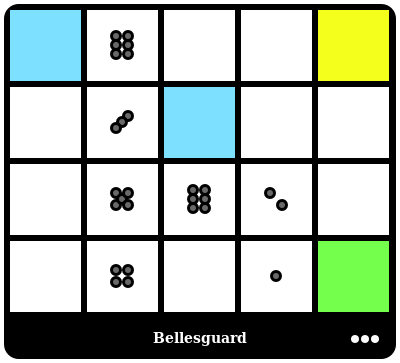
\includegraphics[width=75mm]{img/WPC/Bellesguard.png}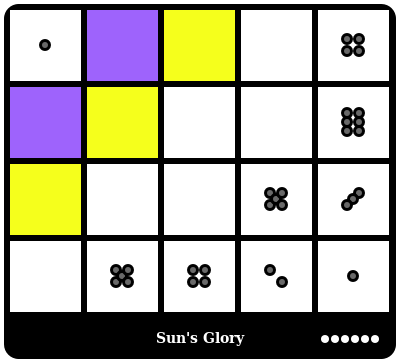
\includegraphics[width=75mm]{img/WPC/Sun'sGlory.png}}}
\centerline{\mbox{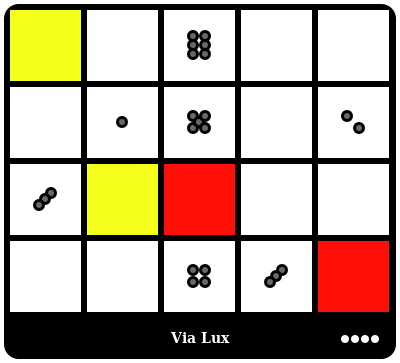
\includegraphics[width=75mm]{img/WPC/ViaLux.png}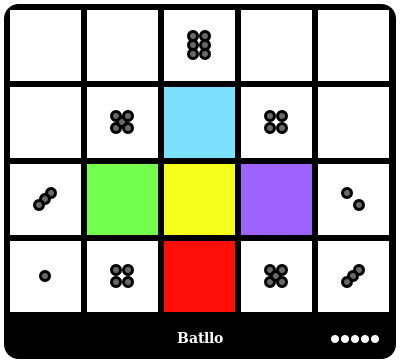
\includegraphics[width=75mm]{img/WPC/Batllo.png}}}
\centerline{\mbox{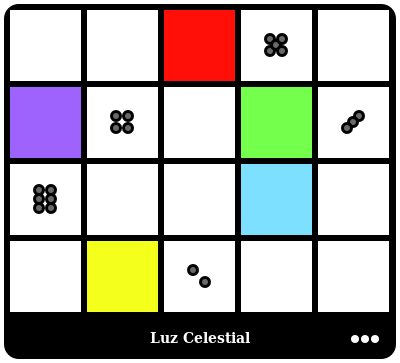
\includegraphics[width=75mm]{img/WPC/LuzCelestial.png}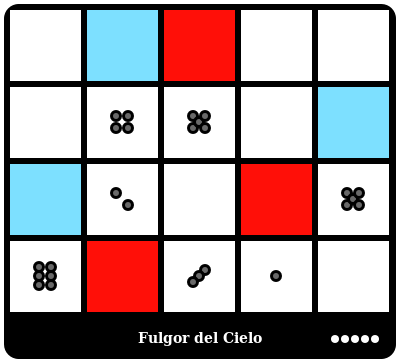
\includegraphics[width=75mm]{img/WPC/FulgordelCielo.png}}}
\centerline{\mbox{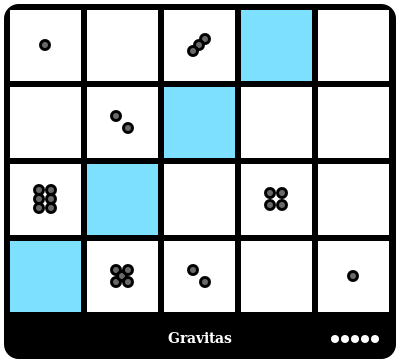
\includegraphics[width=75mm]{img/WPC/Gravitas.png}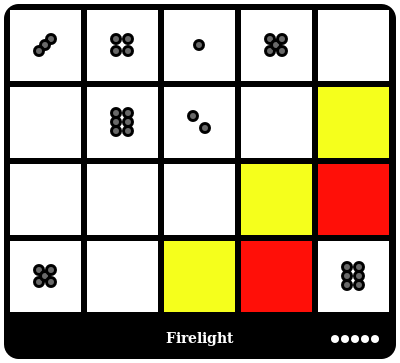
\includegraphics[width=75mm]{img/WPC/Firelight.png}}}

\chapter{Game Analysis}

In this chapter, I will describe Sagrada from a game-theoretic perspective. 


\begin{description}
    \item[Asymmetric] In asymmetric games, players may have different strategies and payoffs. In Sagrada, this occurs by each player having
    a different Private Objective Card that way receiving extra points for different colored dice.
    
    \item[Non-Zero-Sum] Non-zero-sum games can have outcomes where all players benefit (or lose) from their decisions. On the other hand, Sagrada
    has competitive elements similar to Zero-Sum games e.g. players might sometimes choose dice more to deny others than to benefit their window.
    
    \item[Finite Game with Known Horizon] A game that ends after a predetermined number of moves is considered to have a finite horizon. In the two-player 
    variant of the game, the game ends after a fixed number of 20 moves by every player taking two turns in each of the 10 rounds.
    
    \item[Information Structure] The game features imperfect information due to hidden private objectives and stochastic information represented by future dice rolls.
    
    \item[Dynamic Aspects] Players make decisions one after another, allowing for a reaction to the preceding move.
\end{description}


\section{Branching Factor}

The \textbf{branching factor} defines the number of possible actions available to the agent at 
each decision point within a search tree. Understanding its importance is paramount, as it extremely influences the computational complexity, efficiency, 
and effectiveness of various search-based algorithms. A higher branching factor exponentially increases the number of possible paths within the search tree.

In search-based algorithms such as minimax and MCTS, the branching factor profoundly impacts the efficiency of the search process. A lower branching factor 
typically leads to more efficient exploration of the search space, as the algorithm can delve deeper into the tree without sacrificing computational resources. 
Conversely, a higher branching factor necessitates shallower search depths or more aggressive pruning strategies to maintain acceptable performance levels.

The branching factor varies throughout the game, influenced by factors such as the stage of the game and the presence of 
different types of tool cards. Some tool cards provide players with straightforward actions, resulting in a consistent 
branching factor of one for each use. In contrast, other tool cards introduce variability in branching factor, as their effects 
may differ based on the current state of the game or player choices. For example, tool cards that allow players to relocate dice 
on a board can dramatically increase the branching factor by introducing a huge amount of possibilities.

I will now introduce two basic AI agents: the Random agent, which chooses moves randomly, and the First agent, selecting the first possible move at each decision point.
The first possible move of the player is determined by the order described in the \texttt{Game::possible\_moves()} in Section \ref{principle:possible_moves} .
The following figure illustrates the average branching factor over 1000 games of the Random and First agents across the rounds of the game.


\begin{figure}[H]
    \caption{ Branching factor across the rounds for Random and First agents}
    \centerline{\mbox{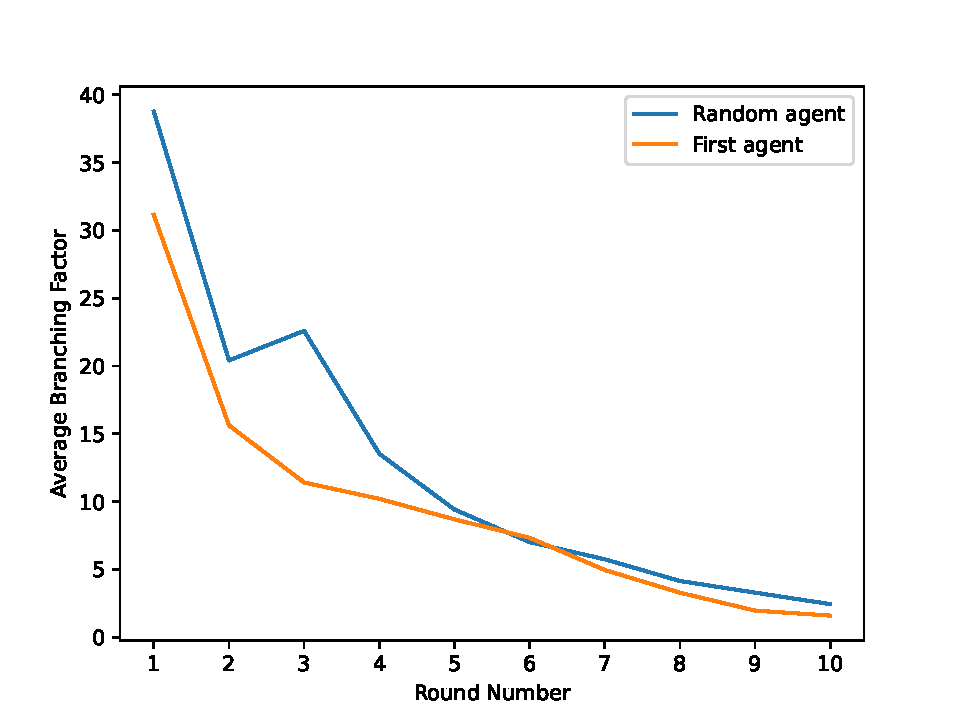
\includegraphics[width=150mm]{img/random_agents_branching_factor.pdf}}}
    \label{fig:example}
\end{figure}


\subsection{Smarter players} \label{subsec:smarter_player_branching_factor}
While these two agents provide a baseline understanding of the branching factor in the game, it's crucial to acknowledge that more strategic or skilled players 
will exhibit different branching factors. Smarter players tend to explore deeper and more selectively within the game tree, leading to a narrower but more focused 
set of potential moves. % An explanation for this phenomenon is that smarter players choose moves that produce uncompletable fields rarely.     

\chapter{Project Structure}

I've created a custom implementation of Sagrada that allows a user to play interactively against 1-3 computer opponents using a graphical interface. 
Additionally, it can simulate games where multiple computer players (2-4) compete against each other, either interactively or through 
a command-line tournament. My implementation does not include the single player variant of the game where a player doesn't have any opponents
but tries to maximize the score with slightly different rules of the game.

\section{OS support}

I developed the game on Ubuntu, and it could potentially be ported to other operating systems such as Windows and other Linux distributions with relative ease, 
although I haven't attempted this. All the frameworks used in this project are cross-platform, enhancing the potential for easy adaptation.


\section{Language and 3rd party libraries}
For this project, the choice of the programming language primarily rested on the need for optimal performance and efficiency. 
I selected C++ as the programming language due to its reputation for producing highly performant code.

The following 3rd party libraries are used in the project:
\begin{enumerate}
    \item gtkmm - gtkmm \cite{gtkmm} is the official C++ interface for the popular GUI library GTK. GTK is widely used for creating graphical user interfaces 
    in applications that run on Linux, Windows, and macOS. I chose this library because it is easy to use, written in C++ and is cross-platform compatible.
    \item nlohmann\_json - an open-source library by Niels Lohmann \cite{nlohmann_json} for parsing JSON objects. It is mainly used for storing game configurations and for unit testing 
    \item argparse - an open-source library used for defining the command line interface \cite{argparse}
    \item googletest - an open-source library used for unit testing \cite{googletest}
\end{enumerate}

\section{Architecture}
The architecture of the system follows the Model-View-Controller (MVC) design pattern, because of its clear separation 
of concerns and scalability. In the MVC architecture, the model represents the application's data and game logic, the view 
handles the presentation layer, and the Controller manages user inputs and coordinates the communication between the model and the view components. 

This separation of concerns is important for many reasons. For instance, our system utilizes the model for different purposes, such as
running games and simulations using the GUI and running tournaments between AI players using the CLI.

\subsection{Model}
The model component is the backbone of the application, responsible for managing data and game logic. Concretely in Sagrada, this means:
\begin{enumerate}
    \item \textbf{Data management} - The model component in Sagrada holds the data about the game including the static data initialized 
    once at the beginning of the game (the different cards, dice, etc.), the current state of the game that is changing (round number, the player on move, etc.)
    and other data that is needed to perform the operations it defines (history of the game).
    \item \textbf{Game logic} - The game logic in Sagrada is represented by the actions that users of the Model component
    perform during the gameplay. These actions include collecting the possible moves, evaluating the sent moves for correctness
    or evaluating the current state of the game.

\end{enumerate}

The main class in the model component is \texttt{the Game class}. It has the following structure:


\begin{figure}[H]
    \caption{ Model structure UML diagram}
    \centerline{\mbox{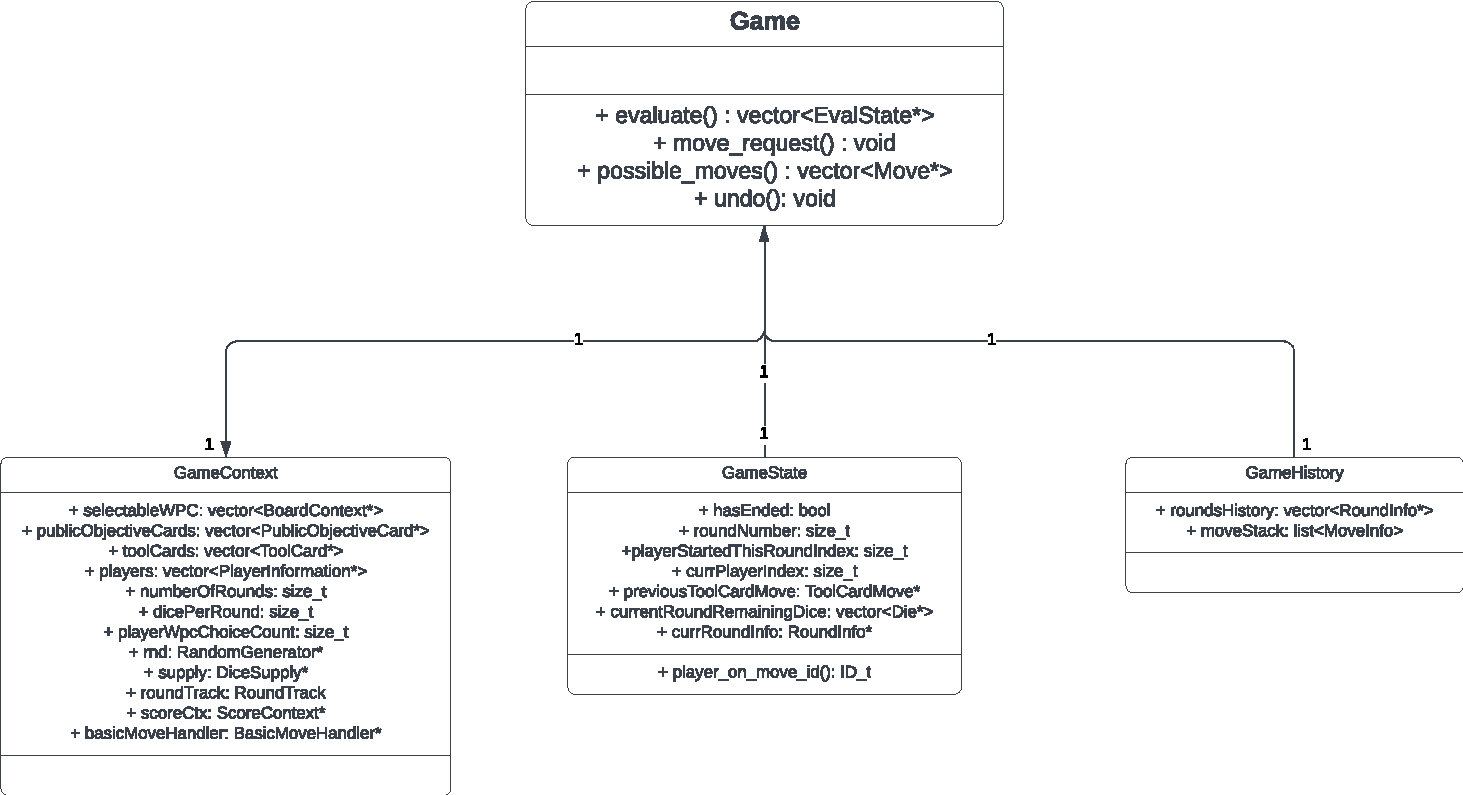
\includegraphics[width=166mm]{img/GameUML.pdf}}}
    \label{fig:Model_UML}
\end{figure}

The reason behind separating the data \texttt{the Game class} holds is connected to avoiding \texttt{the Game class} becoming a God object and following
design principles to achieve a higher factor of flexibility, maintainability and scalability.
\begin{description}
    \item[\texttt{GameContext}] This class represents the static data in \texttt{the Game class} class. Its components are once configured and 
    never changed after. The separation makes \texttt{the Game class} ' API smaller because creating these objects is the responsibility of the GameContextBuilder class.
    Also, it makes \texttt{the Game class} easily configurable by creating a \texttt{GameContext} instance and passing it to the constructor.
    \item[\texttt{GameState}] Dynamically changing data about the current state of \texttt{the Game class} . Having this class independently 
    also has reasons connected to making the API of \texttt{the Game class} smaller and bringing higher scalability.
    \item[\texttt{GameHistory}] Defining the Undo operation requires remembering the actions that lead to a given state of the class to be 
    able to reproduce past states. This class holds the data required for filling this functionality.
\end{description}

As illustrated on Figure \ref{fig:Model_UML} , \texttt{the Game class} has the following most important methods:

\begin{description}
    \item[\texttt{vector<Move*> possible\_moves()}] \label{principle:possible_moves} Returns the vector of all possible moves that are available for the current player at the current state. These
    moves include die-placing moves, Tool Card moves and a Pass move. First, if the previous move of the current player was a Tool Card move that consists
    of multiple sub-moves and there is a way to continue, the sub-moves that are the continuation of the previous sub-move are added. Second, if the player
    has enough favor tokens to use a Tool Card, the Tool Card moves are appended. After that, the die-placing moves are appended starting with dice on the lowest
    index in the \texttt{GameState::currentRoundsRemainingDice} container and the placing board indices are indexed starting from the upper left corner row-wise.
    Finally, the Pass move is added as the last move.
    \item[\texttt{void move\_request(move\_t move)}] Receives a move as an argument and checks whether it is a correct move or not. 
    \item[\texttt{void undo()}] Performs undo operation on the last move. This function is mainly used by AI agents like the minimax agent to produce better 
    performance than cloning every time \texttt{the Game object} a move is about to be evaluated.
    \item[\texttt{vector<EvalState*> evaluate()}] Evaluates the current game state for each player and returns a vector of \texttt{EvalState} objects. This function is called
    at the end of the game for final evaluation and by AI agents for evaluating the state after using given moves. 
\end{description}



\subsubsection{Moves} \label{subsec:Move_Implementation}
The different moves in the game are represented by derived classes from the Move class. Many Tool Cards define their
moves separately derived from ToolCardMove. There are two Tool Cards that consist of multiple sub-moves. The reason behind separating a single move
into multiple sub-moves is that these cards contain randomness meaning that a player chooses to use these Tool Cards, after the first sub-move the new random
value is revealed, and the second sub-move places the new die onto a field if possible. Concretely, these are the mentioned two Tool Cards:
\begin{enumerate}
\item \textbf{Flux Remover} - The first sub-move chooses a die from the Draft Pool to be swapped and swaps it with a die from the Bag. The second
sub-move chooses a value for the die from the Bag and places it onto a field if possible.
\item \textbf{Flux Brush} - The first sub-move chooses a die from the Draft Pool and re-rolls it. The second sub-move places the die onto a field.
\end{enumerate}

\subsection{View}

In this section, we're exploring the view component. I've chosen \texttt{gtkmm3-0} for its ease of use, cross-platform compatibility, and because it's written in C++.
The GUI is structured into pages. Each page in the GUI is equipped with widgets to fulfill specific functions. The two most important pages are the following:
\begin{itemize}
    \item \textbf{GamePlayingPage} - This page is a base class for \texttt{the LocalGamePlayingPage class} and \texttt{the SimulationGamePlayingPage class} 
    since these two pages have the same functionalities except for some user interactions. It displays all the elements of the game such as the boards 
    of the players or the current round's dice.
    \item \textbf{LocalGamePlayingPage} - This page is used when the user chooses to play against AI agents. This page has some specific functionalities 
    other than its base \texttt{class GamePlayingPage}.  These functionalities include selecting a die and placing it onto the player's board or using the Tool Cards.
    \item \textbf{SimulationGamePlayingPage} - This page is used for displaying simulations between AI agents. It is useful when during an experiment a game
    has strange results and we would like to check the steps each AI agent made leading to the odd result.
\end{itemize}



\subsection{Controller}

The Controller component serves as the intermediary between the model and the view components. It primarily handles user input, processes requests, 
and provides appropriate responses. Concretely in Sagrada, the Controllers manage the AI players and forward the human players' move requests in games with human players.

\texttt{The ControllerWithAIPlayer class} serves as a base class for the two concrete controllers.
It stores a reference to the game that is being played and stores the AI players by the corresponding player IDs. 

For playing games with human players, an instance of \texttt{the LocalPlayerController class} is used. This class is derived from 
\texttt{the ControllerWithAIPlayer class} making it able to play games with both human and AI Players. Additionally, it stores the IDs of all
human players providing easier handling for the view components. 

Games that are played between only AI players use an instance of \texttt{the OnlyAIPlayerController class} . This class is used mainly in the Tournament framework.  

\section{Tournament Framework}

Having the Tournament framework independent from the GUI makes experimenting faster and easier. This way it is possible to 
automatize running the different tournaments and processing their results by scripts. To run tournaments, run the 
\texttt{build/tournament} executable. It accepts the following arguments:

\begin{description}
    \item[-h] Displays help information. \\
    \item[-v] Prints the results to the standard output game-by-game. This option is turned off by default.\\
    \item[-s] The starting seed of the tournament i.e. the seed of game 1. The default value is 779. \\
    \item[-n] The number of games in the tournament. There is no default value for this option and it is required to specify one.\\
    \item[-d] Makes the games in the tournament deterministic i.e. all the information is available for all the agents including dice in the upcoming rounds and other players' Private Objective Cards. This option is turned off by default.\\
    \item[-p] The agents that will play against each other in the tournament. This option accepts 2-4 parameters and has no default configuration but it is required to be defined.
    \begin{description}
        \item[random] - An agent choosing a random move
        \item[first] - An agent choosing the first possible move
        \item[rules-based] - An agent with rules-based strategy. \\Example config: rules-based-strategy=only\_dtfm
          \begin{description}
            \item[strategy] Choose a strategy for the player. The two possible options are \textbf{only\_dtfm} and \textbf{all\_moves}
          \end{description}
        \item[minimax] - Minimax agent. \\ Example config: minimax-depth=3,worlds=8,config\_file=config.json
          \begin{description}
            \item[depth] Sets the depth for the minimax search.
            \item[worlds] Sets the determinizing world count.
            \item[config\_file] Sets a config file with heuristic constants.
          \end{description}
        \item[mcts] - Monte Carlo Tree Search agent. \\Example config: mcts-it=120,expl=0.7,worlds=6,playout=random
          \begin{description}
            \item[it] Sets the iteration count for the algorithm.
            \item[worlds] Sets the determinizing world count.
            \item[expl] Sets the exploration constant for the algorithm.
            \item[playout] Sets the playout strategy for the simulation step of the algorithm.
          \end{description} 
      \end{description}
    
    \item[-mode] The mode of the game. Allows the users to run tournaments with a custom configuration. The default value is ``default''.\\
    \item[-b] Runs all the permutations of players in a game using a given seed. This option is turned off by default.\\
    \item[-csv] An option to save the results of the game into a directory of CSV files. The parameter is the name of the directory. This option is turned off by default.\\
    \item[-ms] An option to save information about the branching factor of each player. This option is turned off by default.\\
    \item[-gi] An option to save additional information for each game such as the Tool Cards or the Public Objective Cards used in the game. This option is turned off by default.\\ 
\end{description}
  
An example of running a tournament of 100 games using 800 as the starting seed between a minimax agent and a rules-based agent:
\begin{verbatim}
$ build/tournament -n 100 -p rules-based-strategy=only_dtfm \ 
minimax-depth=4,worlds=4 -s 800 -v
\end{verbatim}
  

When the tournament ends, the framework prints statistics about the game and the players either to the standard output or to the specified CSV files. The statistics include
the number of games won by each player, the average time it took for each player to make a move and the Wilson confidence interval for the tournament-winning player.

A random seed is a number used to initialize a pseudorandom number generator. By setting this seed, the starting point for a sequence of pseudorandom numbers
is determined. This means that changing this random seed for a game results in another game configuration and that way another gameplay. On the other hand,
this also means that using the same seed multiple times produces the same output. The tournament framework uses the random seed received from the command-line
and increases it by one after every game. This means that if the first game used the random seed 779, the second one will use 780 and so on.

There is an option to simulate games played between AI agents using the GUI. This comes in handy if some games produce an interesting outcome in the tournament and the user
would like to check the choices of the AI agents one by one. The CLI is designed to make this task as user-friendly as possible. To simulate a game
that was run in the tournament using the following command:
\begin{verbatim}
$ build/tournament -n 100 -p rules-based-strategy=only_dtfm \
minimax-depth=4,worlds=4 -s 800 -v
\end{verbatim}

run the following command:

\begin{verbatim}
$ build/sagrada simulation -p rules-based-strategy=only_dtfm \
minimax-depth=4,worlds=4 -s 800 -v
\end{verbatim}
  

% \section{Data Processing Scripts}

% This section describes how the given scripts work with the results of the tournaments. The scripts are written in Python
% and I am using different tools to visualize the results of given experiments such as matplotlib or prettytable. The overall
% structure of the data flow is illustrated in the following diagram:


% \begin{figure}[H]
%     \caption{ CSV data flow UML diagram}
%     \centerline{\mbox{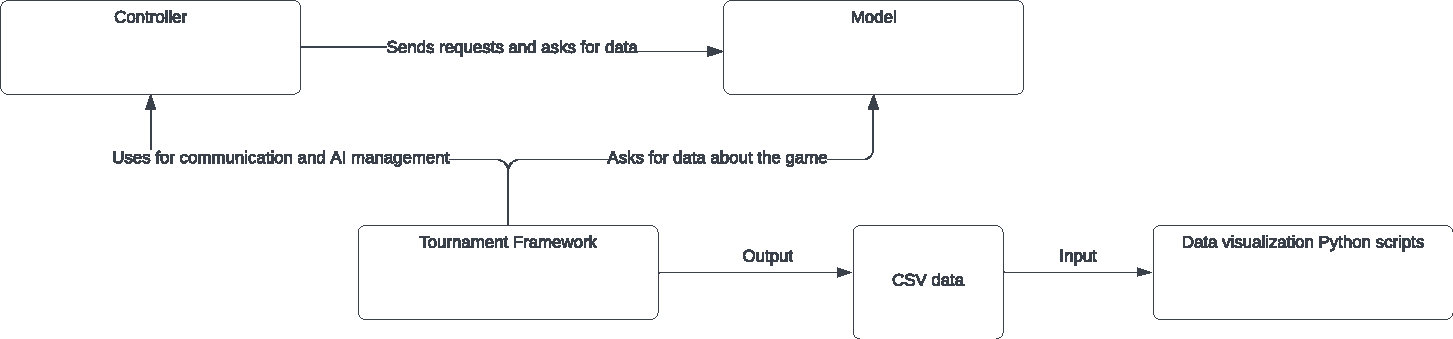
\includegraphics[width=166mm]{img/CSVDataFlow.pdf}}}
%     \label{fig:example}
% \end{figure}


\chapter{Building Blocks for AI Agents}

\section{Board Evaluation}

When implementing an AI agent for games, especially strategy-based ones like Sagrada, the ability to evaluate the 
game board accurately is paramount. This evaluation serves as the foundation upon which the agent makes its decisions, 
determining the quality of its moves. By evaluating the board, the AI agent can 
prepare for future developments and plan its moves accordingly. It can identify key objectives, assess potential risks, 
and devise multi-step strategies to achieve its goals.  Evaluating the board efficiently is crucial for ensuring that 
the AI agent can process information and make decisions under a given time limit. 

\subsection{Board Evaluation in Sagrada} \label{subsec:Board_Evaluation_In_Sagrada}

Evaluating players' boards is one of the functionalities of the model component. The EvalState class is responsible for evaluating
the state of a given player including a board evaluation and the points for the unused favor tokens. Each EvalState object contains
the following components:
\begin{itemize}
    \item The penalty points received for the empty fields
    \item The number of Private Objective Card points received by the player
    \item A vector of PuocPatternState objects each representing the state of a concrete Public Objective Card
    \item The final score of the player that represents the number of points that the player would have if the game had ended before the evaluation
\end{itemize}


\subsubsection{PuocPatternState}
PuocPatternState objects represent the state of a board from the perspective of a given Public Objective Card. These objects
are constructed by the Public Objective Cards during the board evaluation. They contain both rules-based information 
(currently earned points) and heuristic-based information (the heuristic state).

The heuristic-based pattern evaluation is divided into completable and uncompletable patterns. The uncompletable
patterns are simply counted but for completable patterns, the number of dice that are missing to complete
the given pattern is remembered as well. This makes the evaluation of given patterns stronger because given agents can reward
placing dice that bring closer patterns to completion. 

The performance of an evaluation function is critical for agents using algorithms such as minimax, particularly in complex games 
such as Sagrada, where the branching factor is high. Certainly, there's often a trade-off between the accuracy and efficiency of an evaluation function. 
One of the inaccuracies occurs when evaluating Public Objective Cards that contain either a row or a column matching for unique dice colors or shades.
The reason behind this behavior is that each row/column is evaluated independently. However, the neighboring rows/columns have an impact on each other.

I will demonstrate this phenomenon in an example. Suppose that one of the Public Objective Cards is the Row Shade Variety. This means that the player is trying
to place dice so that each row will contain dice with unique shades. The following figure shows an example state:


\begin{figure}[H]
    \caption{ Incorrect evaluation board position example}
    \centerline{\mbox{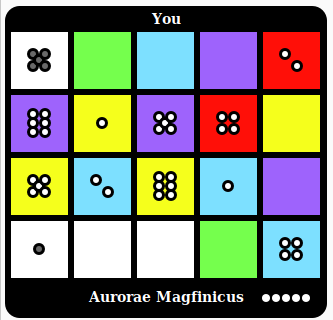
\includegraphics[width=100mm]{img/IncorrectBoardEvaluationExample.png}}}
    \label{fig:example}
\end{figure}


Notice that the second row could be completed with a 2 or a 3, and the third row could be completed with a 3 or a 4. Since the first row
contains a red die with the value of 2 at the rightmost column, a die having a value of 2 cannot be placed to the neighboring fields so the only 
value left for completing the second row is 3. The same principle applies to the third row and the blue 4 die in the fourth row. This means that 
both rows can be completed only with a 3 which is not possible at the same time because of the rules of the game. However, the board evaluation processes the rows
independently so it will report that both of these rows can be finished at the same time. The reason for not implementing it perfectly is connected
to performance. This phenomenon occurs rarely and avoiding it would require looking for a concrete placing of dice to each empty field. I decided 
that implementing this feature would not be worth the performance overhead.


\section{Heuristic Filter} \label{sec:Heuristic_filter}

Heuristic filters play a crucial role in AI algorithms, particularly in scenarios where exhaustive search or perfect evaluation is impractical due to 
computational constraints. Heuristic filters help narrow down the search space by quickly discarding unpromising choices, allowing the AI algorithm to 
focus its computational resources on more promising alternatives. 

One common pitfall is inadvertently limiting future placement options by positioning dice in a way that conflicts with the game's color or shade restrictions. 
Recognizing this, a heuristic filter can be employed to identify and avoid such ``bad moves'', both in regular die-to-field placements and when using Tool Cards.
When considering potential moves for placing a die on the board, the heuristic filter evaluates each option to determine if it would place a die adjacent to a field 
that shares the same color or shade restriction as the placed die. If such a placement is found, it's flagged as undesirable and filtered out. 
By proactively avoiding these conflicting placements, the AI ensures that it maintains flexibility and maximizes its future placement opportunities.
Similarly, when using Tool Cards, the heuristic filter explores the potential outcomes of each action to identify any placements that would create conflicts with 
existing dice on the board.

The Heuristic Filter is implemented in \texttt{the HeuristicFilter.h header file} that is part of the AI code of the project. The main function is the 
\texttt{void filter\_moves(Game\&, const vector<Move*>\& allMoves, vector<Move*>\& bestMoves, vector<Move*>\& backupMoves)} that receives all the moves to be filtered
and separates them into the \texttt{bestMoves} and \texttt{the backupMoves containers} using the filtering policy defined above.
The ``backup moves'' are used when there are no ``good moves'' to work with.

This technique is called ``forward pruning'' in the popular AI textbook \cite{norvig2002modern} . They say that ``Forward pruning prunes moves that appear to be poor moves, 
but might possibly be good Forward pruning ones. Thus, the strategy saves computation time at the risk of making an error''.

The following figure illustrates the impact of the Heuristic filter presented by the two AI agents that use it:
\begin{figure}[H]
    \caption{The impact of the Heuristic filter on the branching factor of two different AI players}
    \centerline{\mbox{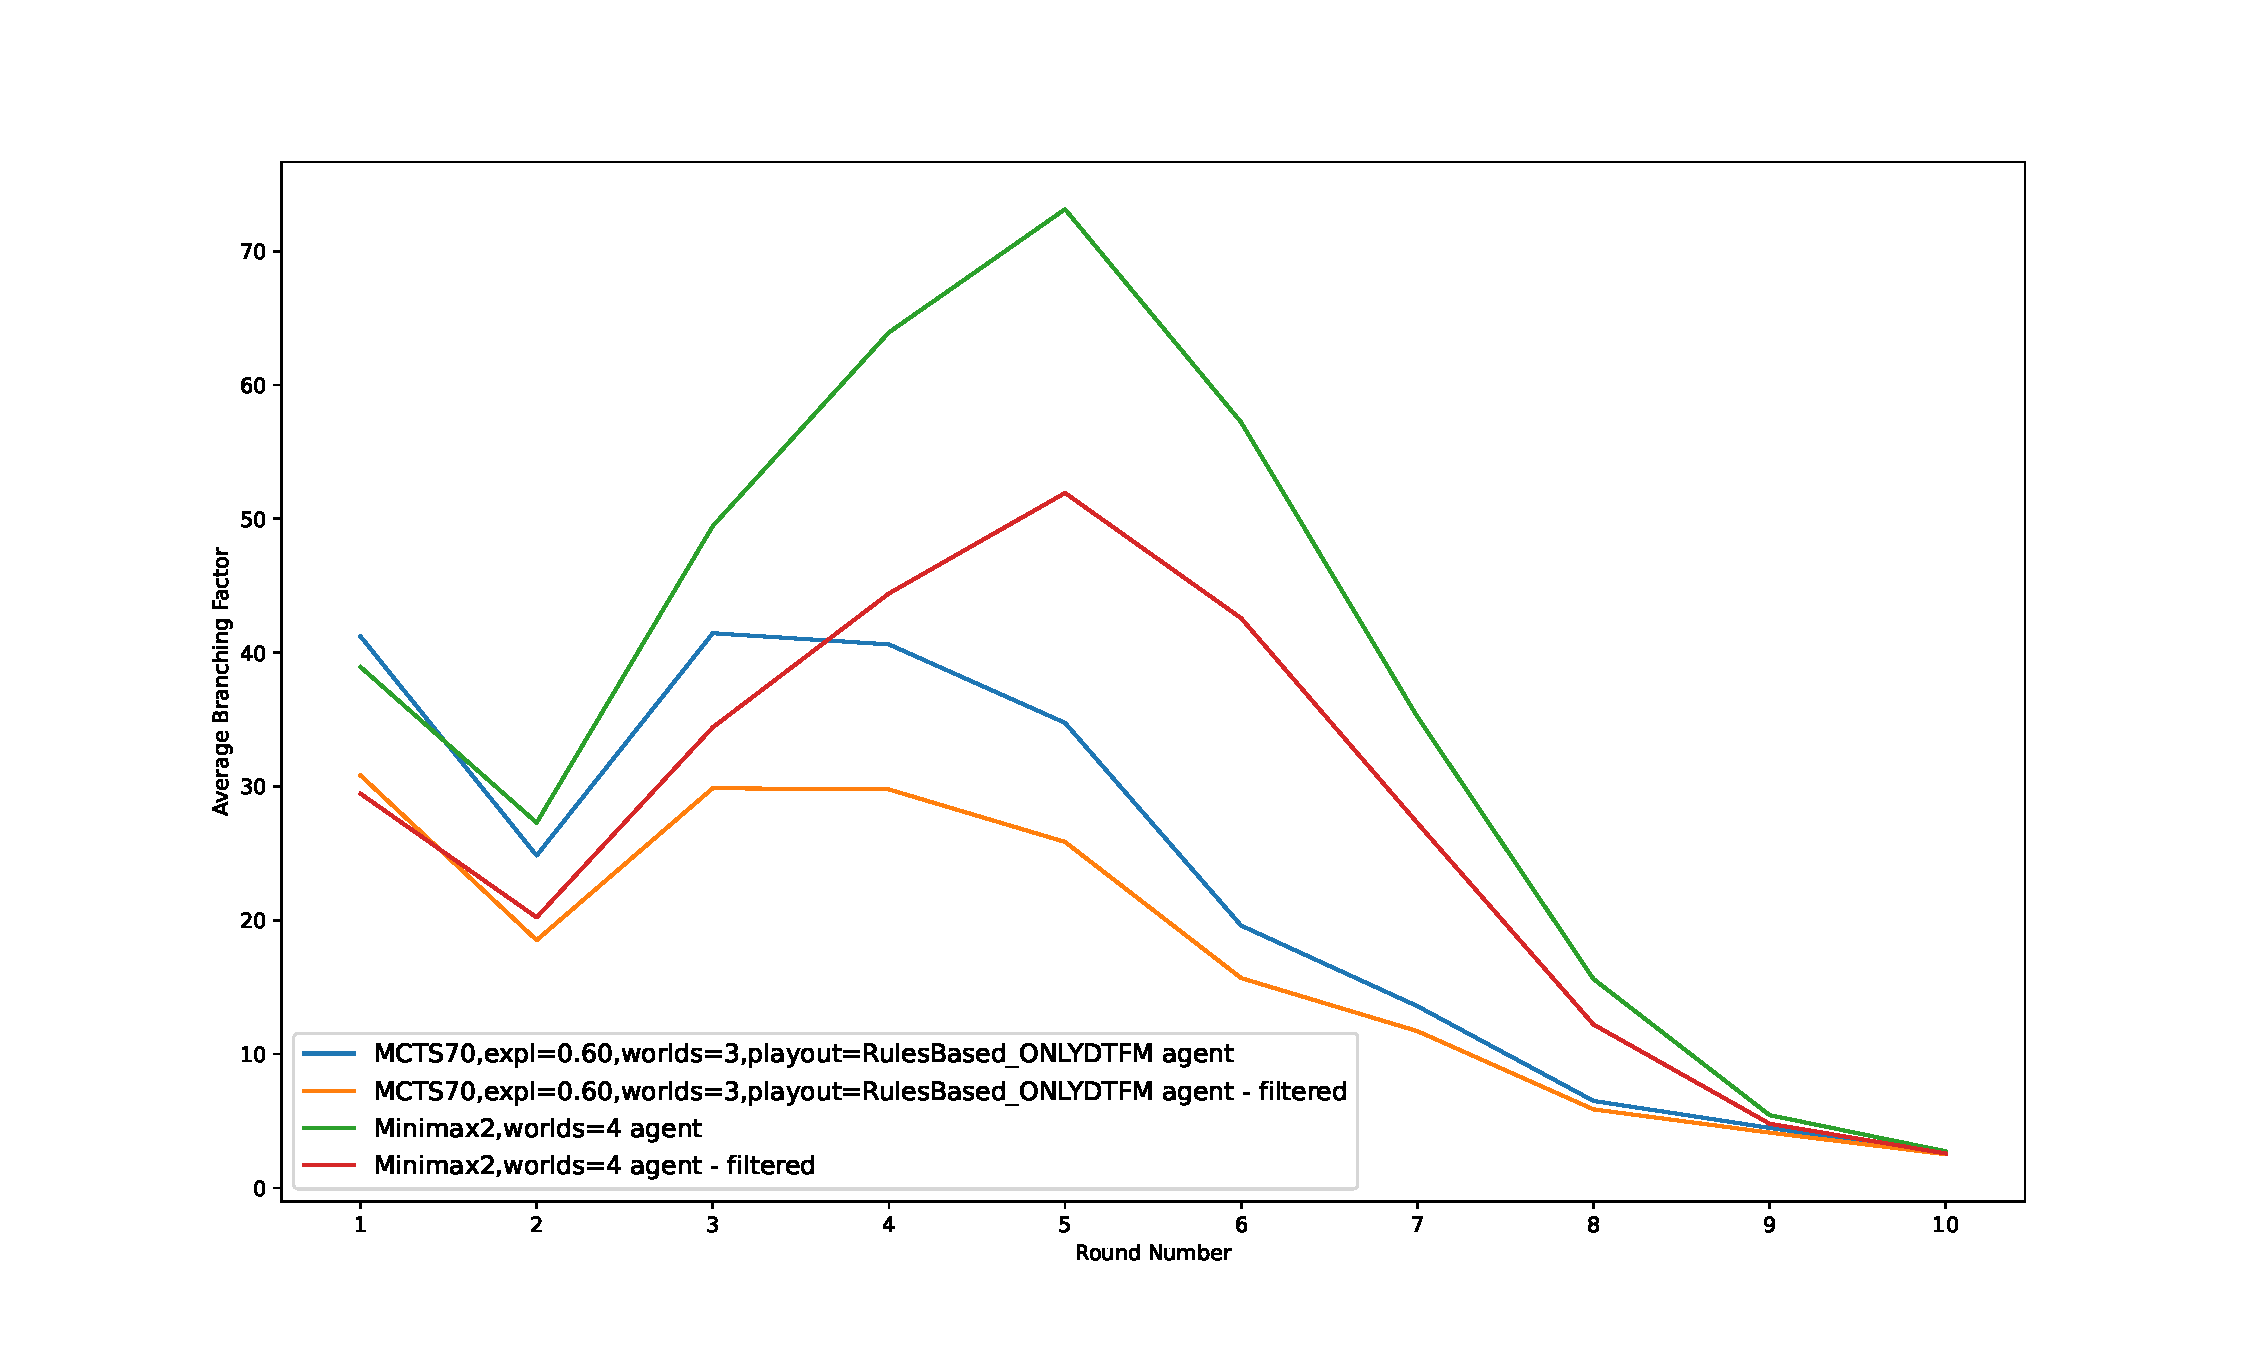
\includegraphics[width=180mm]{img/heuristic_filter.pdf}}}
    \label{fig:example}
\end{figure}

\section{Heuristic Sort} \label{sec:Heuristic_sort}

Heuristic sorting of moves plays a pivotal role in modern AI algorithms for board games, providing a strategic advantage by guiding the AI agent towards more promising moves. 
Furthermore, heuristic sorting facilitates the exploration of deeper and more complex game trees within a limited computational budget. In games with high branching factors, 
heuristic sorting allows AI agents to efficiently allocate their resources towards exploring the most promising branches of the game tree. Since the comparator is executed numerous times, 
its efficiency is critical to ensure the overall speed and responsiveness of the sorting algorithm.

In the previous section, I have already talked about filtering the least promising moves. This section provides a deeper understanding of how the remaining moves are sorted.
Due to the time limit, we cannot use any heuristic-based sorting technique that would be connected to the Public Objective Card patterns. There is one component in the scoring
structure that is easy to use as the basis of the sorting algorithm, namely the Private Objective Card's color.

The sorting algorithm decides between two moves according to the following criteria:
\begin{enumerate}
    \item If none of the moves is a die-placing move, a random move is prioritized
    \item If one of the moves is a die-placing move and the other one is not, the die-placing move is prioritized. 
    \item If one of the dice matches the color of the Private Objective Card and the other does not, the die matching the Private Objective Card color is prioritized.
    \item If one move places a die to a field that has a restriction and the other one does not, the one placed to a field with a restriction is prioritized.
    \item Finally, the die with the higher value is prioritized.
\end{enumerate}

The Heuristic Sort is implemented by \texttt{the comparator functor MoveHeuristicCMP} that is part of the AI code. It is designed to be used with \texttt{the std::sort algorithm} 
from the standard library as the comparator function.
\chapter{Minimax Agent}

In the world of artificial intelligence and game strategies, the minimax algorithm is a key method for making decisions when competing against others.
The main idea of minimax is to predict and counter the opponent's moves while trying to maximize its own advantage.
At its core, the minimax algorithm operates on the principle of recursively exploring the game tree, considering all possible moves by both players 
up to a certain depth or until a terminal state is reached. Each node in the tree represents a game state, and the algorithm assigns a value to 
each node based on the potential outcome of the game from that state. The key idea driving minimax is the assumption that the opponent will make 
moves that are optimal for them, aiming to minimize the agent's potential gain.

While minimax is powerful, it is also a heuristic-based approach. It doesn't guarantee finding the optimal solution but rather approximates it by 
searching through the game tree. Despite its effectiveness, minimax does have limitations, primarily related to the vast branching factor of certain game trees, 
which can lead to exponential growth in computation as the depth increases. 

While minimax excels in deterministic games like chess, its application becomes more complex in games with imperfect information, 
where players have limited or incomplete knowledge about the game state or their opponents' actions. In non-deterministic games, traditional minimax 
strategies struggle due to the inability to accurately assess the state space. Unlike deterministic games where the entire game state is known, 
non-deterministic games introduce uncertainty, making it difficult for the agent to construct a comprehensive game tree.

In this chapter, I delve into the implementation of minimax specifically adapted for Sagrada. I discuss how I approached challenges such as 
high branching factors and imperfect information within the context of Sagrada's gameplay mechanics. By detailing my approach to integrating minimax into 
the game's decision-making process while addressing these factors, I aim to provide valuable insights into the development of AI agents for complex board games.

\section{Branching Factor}

As discussed in Section \ref{subsec:smarter_player_branching_factor} , it's evident that smarter players exhibit markedly different branching factors compared to random agents.
In the case of minimax agents, the branching factor tends to be significantly higher because the heuristic function guides the player towards more promising moves. This results
in choosing moves that make space for higher branching factor in the following turns because it rarely chooses moves that produce uncompletable fields and fields that 
are completable with only a small amount of different dice. The following figure visualizes the average branching factor over 1000 games for a minimax and a random agent:

\begin{figure}[H]
    \caption{ Branching factor comparison between the minimax agent and the random agent}
    \centerline{\mbox{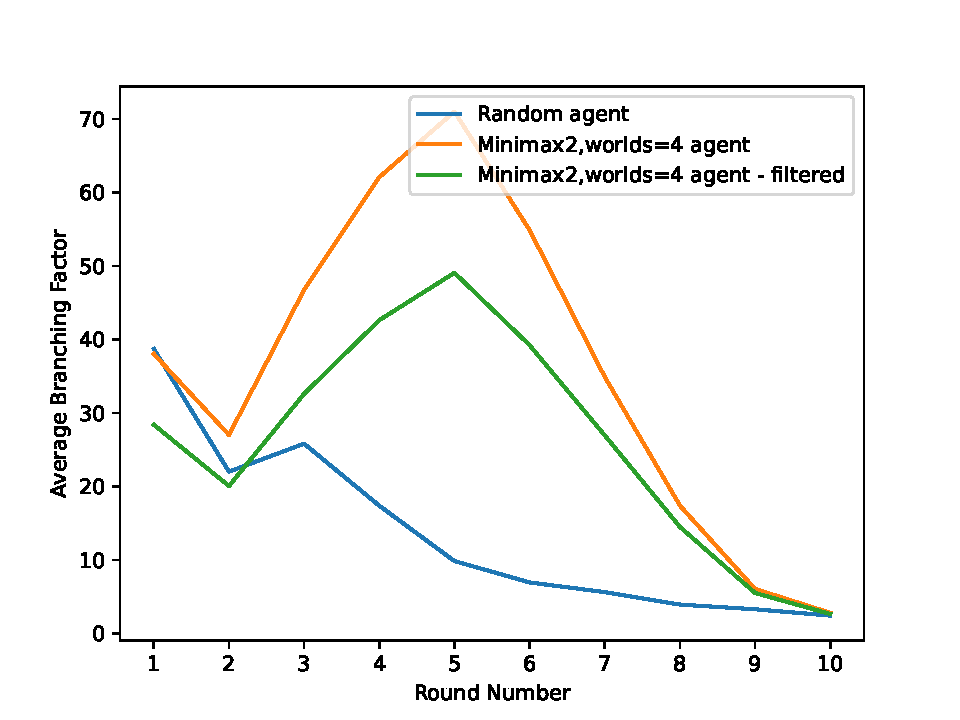
\includegraphics[width=180mm]{img/minimax_agent_branching_factor.pdf}}}
    \label{fig:example}
\end{figure}


\section{The Algorithm}

At its core, the minimax algorithm operates on the premise of minimizing the possible loss for a worst-case scenario while simultaneously maximizing potential gains. 
It's particularly effective in two-player, zero-sum games, where each player aims to outmaneuver the other. 

The game's possible future states are represented as a game tree, with each node denoting a possible move by a player. In Sagrada, a game with a high branching factor, 
this tree can rapidly expand, making exhaustive search impractical.  Each terminal node or leaf of the game tree is assigned a heuristic value, 
reflecting the desirability of that game state for the player. Starting from the terminal nodes, these values are propagated upwards through the tree. 
Generally, at each level, the algorithm alternates between maximizing and minimizing the values, simulating the moves of both players. 
For a comprehensive overview of the minimax algorithm, see \cite{enwiki:1217764079}.


This works for games where the players make moves one after the other. Note that in Sagrada choosing the minimizing and the maximizing player for the next layer is not 
that straightforward because the players do not strictly alternate moves. Also, the implementation of some Tool Cards consists of multiple sub-moves as described in Section 
\ref{subsec:Move_Implementation}  making the choice of the next level's playing strategy even harder. 

To explore the state nodes of the game tree, I am using the pre-processed possible moves using the heuristic filter already described in Section
\ref{sec:Heuristic_filter} . This is one of the ways I am dealing with the high branching factor.

Finally, the algorithm selects the move that leads to the highest possible outcome assuming optimal play from both players. 
This move is the one most likely to maximize the player's payoff while minimizing the opponent's.

Thanks to the implementation of the undo operation of \texttt{the Game class}, trying out moves becomes 
fast since instead of cloning \texttt{the Game object} for each move, we simply make a move and then at the right time, we undo it. 

\subsection{Alpha-Beta Pruning}

While the minimax algorithm is powerful, its effectiveness can be hampered by the sheer size of the game tree, especially in games like Sagrada with a high branching factor. 
Alpha-beta pruning is a technique used to reduce the number of nodes evaluated by the minimax algorithm. It works by cutting off branches of the game tree that are guaranteed to be unfruitful. 
In essence, it prunes away portions of the search tree that need not be explored further, significantly reducing the computational overhead. A detailed explanation of 
alpha-beta pruning is available on its Wikipedia page \cite{enwiki:1198585667}.


In my implementation, after the moves are filtered according to the description in the previous section, the remaining moves are sorted using the heuristic sort comparator described in Section 
\ref{sec:Heuristic_sort} . When the moves are selected in the sorted order, they are processed one by one. Processing the most promising moves first makes
the alpha-beta pruning effective.

\subsection{Handling Imperfect Information} \label{sec:Minimax_Handling_Imperfect_Information}

When utilizing a minimax agent with a depth parameter greater than 1 in Sagrada, the agent has to deal with handling stochastic information, particularly 
regarding the dice available in future rounds.  One option for handling this situation easily would be simply not allowing the minimax player to go beyond the current round. 
This technique is easy to implement but I chose to experiment with a more complex solution. 

Another way of handling imperfect information is to make different worlds where all the information is deterministic and available for all the players. This approach
creates different worlds by choosing a concrete random value for every hidden and non-deterministic information in the game. When the worlds are created, the algorithm 
is run in each of them. After the algorithm has finished in every world, the sub-results are combined to make a final move. 

Selecting a fixed number of deterministic worlds to create is non-trivial. For this reason, the number of worlds created is given by a parameter to the minimax player
making it possible to experiment with different world counts. 

\subsection{Final Move Selection} \label{subsec:Minimax_Final_Move_Selection}

The final move that is chosen by the minimax agent is the one that has shown the best behavior across all the determinized worlds. To achieve this,
there is a vector of move-heuristic value pairs filled with the first layer's pairs. Notice that the first layer contains only deterministic
information because the current round's dice are always revealed. This means that all the worlds have the same moves on the first layer which are 
the possible moves of the agent itself. All this helps to combine the results of the worlds to a final decision by adding together the heuristic values
at the same index obtained from the worlds. After combining the sub-results, I simply choose the one with the highest combined heuristic values.

\begin{algorithm}[H]
    \caption{Minimax algorithm}
    \begin{algorithmic}[1]
        \Function{make\_next\_move}{}
            \State $combinedWorldResults \gets []$
            \For{$i \gets 1$ \textbf{to} $worldCount$}
                \State $sampleWorld \gets game.clone\_with\_random\_future() $
                \State $currWorldResults \gets [] $
                \State \Call{minimax\_algorithm}{sampleWorld, depth, INT\_MIN, INT\_MAX, maximizingPlayer, currWorldResults}
                \State $combinedWorldResults \gets $
                \State \hspace{\algorithmicindent}$combine\_results(combinedWorldResults, currWorldResults) $
            \EndFor
           
            \State \textbf{return} the move with the highest combined heuristic value
        \EndFunction

        \Function{minimax\_algorithm}{gameWorld, depth, alpha, beta, player, firstLayerResults}
            \If{$ depth == 0$ \textbf{or} $gameWorld.has\_ended $}
                \State \textbf{return} {NULL, heuristic(gameWorld)}
            \EndIf

            \State $allMoves \gets $ \Call{gameWorld.possible\_moves}{ }
            \State $bestMoves, backupMoves \gets$ \Call{filter\_moves}{gameWorld, allMoves}
            \If{$bestMoves.empty()$}
                \State $bestMoves \gets backupMoves$
            \EndIf

            \State \Call{sort}{bestMoves, MoveHeuristicCMP}
            \State $currBestPlayerVal \gets player.get\_initial\_value() $
            \For{$\text{move}$ \textbf{in} $\text{bestMoves}$}
                \State \Call{gameWorld.move\_request}{move}
                \State $nextLayerPlayer \gets\ get\_next\_layer\_player() $
                \State $retMove, heuristicVal \gets $ \Call{minimax\_algorithm}{gameWorld, depth-1, alpha,beta, nextLayerPlayer, NULL}

                \If{$firstLayerResults$ \textbf{not} $NULL$}
                    \State $firstLayerResults.add(retMove, heuristicVal)$
                \EndIf

                \State \Call{gameWorld.undo\_last\_move}{ }
                \If{$player.is\_better\_value(heuristicVal, currBestPlayerVal)$}
                    \State $currBestPlayerVal, bestMove \gets heuristicVal, move $
                \EndIf

                \If{$beta <= alpha$}
                    \State \textbf{break}
                \EndIf
            \EndFor

            \State \textbf{return} {bestMove, currBestPlayerVal}
        \EndFunction
    \end{algorithmic}
\end{algorithm}



\section{Heuristic Function} \label{sec:Minimax_Heuristic_Function}

In the context of the minimax algorithm, the heuristic function plays a pivotal role in guiding the agent's decision-making process within the search tree.
The quality of the heuristic function directly impacts the efficiency and effectiveness of the minimax algorithm. A well-designed heuristic can effectively 
prune branches of the search tree, focusing the agent's attention on promising moves and significantly reducing computational overhead. 


Introducing two values, \texttt{HEURISTIC\_MIN} and \texttt{HEURISTIC\_MAX} are the smallest and the greatest values defined for the heuristic value of a game state.
My heuristic function in Sagrada is divided into two parts: evaluating games that have already ended and all the other game states.
I will begin by introducing the simpler case, evaluating a game that has already ended. In this scenario, the heuristic function returns \texttt{HEURISTIC\_MIN} if the agent
lost, \texttt{HEURISTIC\_MAX} if the agent won. 

Computing the heuristic value of a given state when the game has not ended yet is more sophisticated. The HeuristicConstants structure
holds constants used in the heuristic function defining weights for different components. The final heuristic value of a state is the weighted heuristic 
value of all the other agents' scores subtracted from the heuristic value of the minimax agent's score. The EvalState object described in Section \ref{subsec:Board_Evaluation_In_Sagrada}  
serves as a basis to calculate the heuristic value of a player's state. 

The heuristic value of a state is computed from 4 components: rewards for the already achieved points, rewards for the completable Public Objective Card patterns,
penalties for uncompletable Public Objective Card patterns and finally penalties for fields where the player won't be able to place a die without using a relocating Tool Card.
Motivating the agent to continue completing patterns closer to completion is important. For this reason, calculating the reward for completable Public Objective Card patterns 
is designed to follow this idea prioritizing the ones with higher satisfaction values. The other 3 components are simply multiplied by the weight gained from the 
HeuristicConstants object. The following pseudocode illustrates the evaluation function:

\begin{algorithm}[H]
    \caption{Minimax heuristic}
    \begin{algorithmic}[1]
    \Function{get\_heuristic\_value\_for\_score}{$score$}
        \State $puocUncompletablePoints \gets 0 $
        \State $weightedPuocCompletable \gets 0 $
        \For{$\text{puocState}$ \textbf{in} $\text{score.puocStates}$}
            \State $sv \gets puocState.satisfactionValue $
            \State $puocUncompletablePoints \gets $
            \State \hspace{\algorithmicindent}$puocUncompletablePoints + (puocState.uncompletablePatternCount * sv)$
            \For{$\text{pattern}$ \textbf{in} $\text{puocState.completablePatterns}$}
                \State $weightedDiceToComplete \gets $
                \State \hspace{\algorithmicindent}$(puocState.dicePerPattern - pattern.diceToComplete + 1)^{puocCompletableWeight} $
                \State $weightedPuocCompletable \gets $
                \State \hspace{\algorithmicindent}$weightedPuocCompletable + sv * weightedDiceToComplete$
            \EndFor
        \EndFor

        \State $weightedCompletedPoints \gets  $
        \State \hspace{\algorithmicindent}$score.completedPoints * completedPointsWeight$
        \State $weightedUncompletablePoints \gets $
        \State \hspace{\algorithmicindent}$puocUncompletablePoints * puocUncompletablePointsWeight $
        \State $weightedUncompletableFields \gets   $
        \State \hspace{\algorithmicindent}$score.boardState.uncompletableFieldCount * uncompletableFieldCountWeight$
        \State \textbf{return} $weightedCompletedPoints + weightedPuocCompletable - weightedUncompletablePoints - weightedUncompletableFields$
    \EndFunction
    \end{algorithmic}
\end{algorithm}

The weight constants \texttt{completedPointsWeight}, \texttt{puocUncompletablePointsWeight}, \texttt{uncompletableFieldCountWeight} and \texttt{puocCompletableWeight}
are the constants from the HeuristicConstants structure.

\chapter{Rules-Based Agent}

Rules-based AI agents in board games operate on predefined sets of rules and strategies programmed by developers. These agents analyze the game state, 
evaluate available moves, and select the best course of action based on a predetermined set of rules. 


My rules-based agents assess the potential moves within the current state but refrain from delving deeper into constructing a comprehensive tree of 
possible game states by exploring multiple move sequences across various depths. This implies that the rules-based agents don't have to deal with
imperfect information since all the information is available at the current state and they don't look beyond the current move.


\section{Only Die To Field Move Strategy}

As the name suggests, this strategy of the rules-based agent makes only moves that place a die onto a field i.e. it doesn't use any Tool Cards.
The main reason for having this strategy is connected to performance because Tool Card moves contribute significantly to the average branching factor.
Agents using this strategy not only don't have to consider using Tool Card moves but they save time by not even generating the Tool Card moves.

The rules-based agents don't use the heuristic filter and the heuristic sort functionalities. The algorithm begins
with saving information about the current state. After this, all the moves are tried out and the new states are compared with the initial one. The 
moves are evaluated using the following criteria:
\begin{enumerate}
    \item \textbf{Minimize the count of newly appearing fields that cannot be filled without using a relocating tool card} - Increasing the count of these fields potentially 
    leads to increasing uncompletable Public Objective Card patterns and empty fields at the end of the game. For this reason, if the algorithm encounters a move that increases
    this number compared to the current minimum, the move is immediately skipped.
    \item \textbf{Public Objective Card state} - I evaluate the state of the game from the perspective of the Public Objective Cards with a very similar heuristic function
    described in Section \ref{sec:Minimax_Heuristic_Function} .
    \item \textbf{Color of the die} - If the color of the die matches the color of the agent's Private Objective Card, the state value is increased by the weighted value
    of the die.
    \item \textbf{Total points achieved} - Finally, the total points achieved are compared to the current best move's total points.
\end{enumerate} 

The algorithm updates the current best move if the processed move shows better results in the Public Objective Card state and the Total points achieved components.


\section{All Moves Strategy}

The algorithm begins with separating all the possible moves into three categories: relocating tool card moves, tool card moves that contain randomness and all the other 
moves including die-placing moves and other tool card moves. First, the relocating moves are processed. The main criterion followed is to choose the move
that makes the number of uncompletable fields the minimum possible. If there is at least one such move, it will be used. Second, using the algorithm described
in the previous section, I evaluate the die-placing moves and all the tool card moves that contain placing a die onto a field as a sub-move. If die-placing move selected by the
Only Die To Field Move Strategy has a positive heuristic value, it will be chosen as the main move. Otherwise, if there are any moves
containing randomness, a random one of these moves will be chosen. Finally, if none of the previous actions led to a final move, the very first possible move will be chosen.

\section{Branching Factors}

To demonstrate the difference in performance, I ran 1000 games between two agents using the two different strategies. The following plot visualizes
the average branching factor over 1000 games:


\begin{figure}[H]
    \caption{ Branching factor across the rounds for the two rules-based strategies}
    \centerline{\mbox{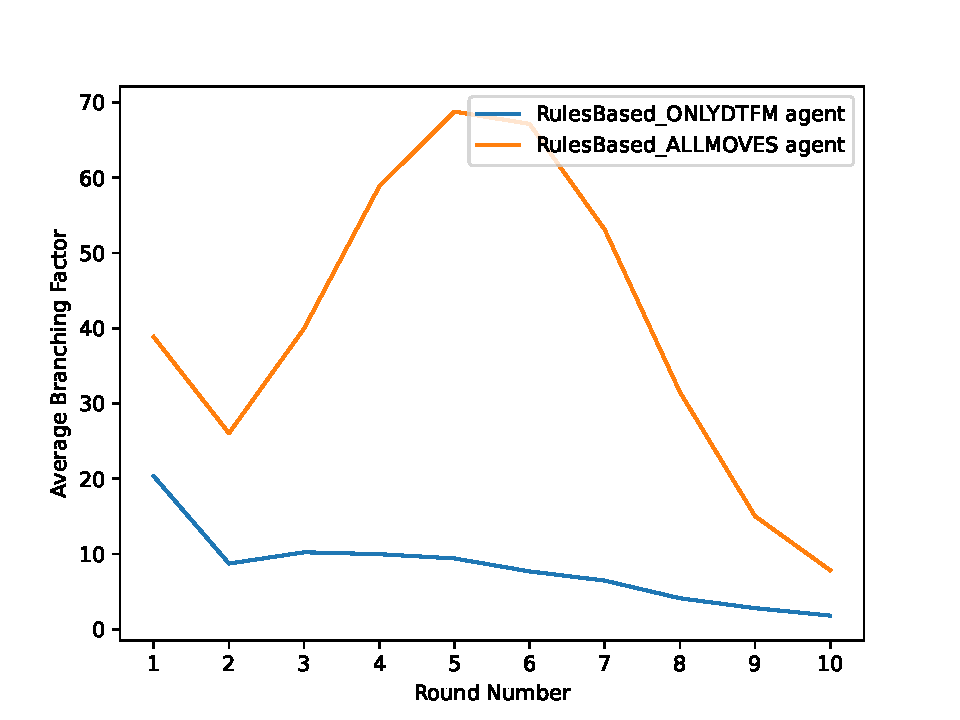
\includegraphics[width=150mm]{img/rules-based_agents_branching_factor.pdf}}}
    \label{fig:example}
\end{figure}

\chapter{Monte Carlo Tree Search Agent} \label{chap:MCTS}

The Monte Carlo Tree Search (MCTS) algorithm is a powerful method that has shown great results in games such as chess or Go. The algorithm
works by building a decision tree and using simulations with different strategies to explore the possible outcomes from the current state. 
It iteratively selects and expands the most promising options based on previous simulation results.

The algorithm is divided into four phases: selection, expansion, simulation, and backpropagation. In the selection phase, the algorithm 
traverses the tree from the root to a leaf node, employing a selection strategy, often based on the Upper Confidence Bound (UCB) algorithm, to choose the 
most promising child nodes. Second, the expansion phase adds one or more child nodes to the selected node, representing possible future states 
of the game. Once a leaf node is reached, playouts from the current state are performed until a terminal state is reached. The outcomes of these simulations 
provide feedback about the value of each child node. In the backpropagation phase, these results are used for updating the rewards of each node along 
the path traversed during selection. For a deeper understanding of the algorithm, I recommend reading the paper \cite{winands2017monte} that specifically describes
the application of the MCTS in board games. 

In this section, our focus shifts to the application of Monte Carlo Tree Search in Sagrada. The nodes have the following structure:

\centerline{\mbox{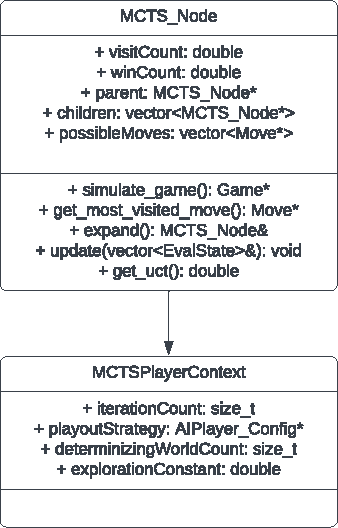
\includegraphics[width=70mm]{img/MCTS_NodeUML.pdf}}}



\section{Selection} \label{sec:MCTS_Selection}

The selection phase in the MCTS algorithm plays a crucial role in efficiently navigating the search tree towards the promising regions while balancing exploration and exploitation. 
One frequently used algorithm for the selection is the Upper Confidence Bound for Trees (UCT) approach being a promising solution for the exploration-exploitation dilemma.

\subsection{Upper Confidence Bound} \label{subsec:MCTS_Selection_UCT}

The UCT formula balances the exploitation of known good actions and the exploration of less explored ones. It calculates the value of each possible action by considering 
both its average reward and the uncertainty associated with it. 

The UCT formula is expressed as:
\[UCT = \bar{X_i} + C \cdot \sqrt{\frac{\ln{N}}{n_i}}\]
where:
\begin{itemize}
    \item $\bar{X_i}$ is the average reward of action i
    \item N is the total number of times the current node has been visited.
    \item ${n_i}$ is the number of times action i has been selected.
    \item $C$ exploration constant balancing exploration and exploitation.
\end{itemize}

Finding an exploration constant that produces the best results possible is not a trivial task. A higher value increases the weight of the exploration term in the formula. 
This leads to more exploratory behavior, as actions that have been sampled less frequently will have a higher UCT value, making them more likely to be chosen.
On the other hand, a lower value of the exploration constant diminishes the influence of the exploration term, thus favoring exploitation. This behavior pushes the 
agent more towards the moves that produced favorable results in the past. A common choice of the exploration factor is $\sqrt{2} $ but in my implementation, I chose
to make the exploration constant a configurable parameter so it was possible to experiment with different constants and compare the results.

The following pseudocode illustrates my implementation of the selection phase:

\begin{algorithm}[H]
    \caption{MCTS Selection}
    \begin{algorithmic}[1]
    \Function{get\_uct}{}
        \State $exploitationFactor \gets winCount / (visitCount \times 5)$
        \State $explorationFactor \gets C \times \sqrt{\frac{\log(parent.visitCount)}{visitCount}}$
        \State \textbf{return} $exploitationFactor + explorationFactor$
    \EndFunction
    
    \Function{select}{$root$}
        \State $currNode \gets root$
        \While{$currNode.is\_fully\_expanded()$ \textbf{and} $!currNode.is\_leaf()$}
            \State $currNode \gets \text{currNode's child that has the highest get\_uct() value}$
        \EndWhile
        \State \textbf{return} $currNode$
    \EndFunction
    \end{algorithmic}
\end{algorithm}


\section{Expansion}

After the selection phase, the expansion step involves adding new nodes to the search tree to explore new parts of the game state space.  If the leaf node is not a terminal state 
and has unexplored actions, the expansion step adds one or more child nodes to the tree corresponding to these actions. Each child node represents a possible action from the current game state.

In my MCTS agent for Sagrada, the moves that lead to new game states represented by the nodes are filtered and sorted using the heuristic filter and the heuristic sort comparator 
described in Sections \ref{sec:Heuristic_filter} and \ref{sec:Heuristic_sort} . For the same reason as in the case of any other agents, these methods are applied to reduce the 
branching factor and to eliminate the weak moves.

\section{Simulation}

The simulation phase, often referred to as playout, is a crucial step in the Monte Carlo Tree Search (MCTS) algorithm where the search tree is traversed from a leaf node to a 
terminal state through a series of simulated gameplays. The primary objective of the simulation phase is to estimate the potential outcome of a game from a given leaf node by 
conducting a series of simulated plays until a terminal state is reached. These simulated plays help in evaluating the quality of the current game state and guide the selection 
of promising actions.

In the simulation phase of the MCTS algorithm, the strategy employed must strike a balance between speed and strength. In my implementation, the playout
strategy of the MCTS player is a configuration parameter that could be changed for different games. This allows experimenting with different strategies to perfect the balance and 
be as strong as possible. Each of the configurable strategies is an AI agent itself such as the Random agent, the Minimax agent or the Rules-based agent.


\section{Backpropagation}

The backpropagation step is responsible for updating the statistics of nodes in the search tree based on the outcome of simulated playouts. This process plays a crucial role in 
guiding the selection towards promising moves. Backpropagation involves updating the statistics of all nodes along the path from the leaf node to the root node. 
The most common technique in backpropagation is to propagate the outcome of the playout (e.g., a win or loss) back up the tree and update the win count and visit count of each node accordingly. 

I decided to use a more sophisticated reward system. The visit count of each node is always incremented by one in the backpropagation phase regardless of the result of the game.
The win count of each node is incremented by 1 if the player wins the game in the simulated playout.  Additional bonuses are awarded based on the player's score differential compared 
to their opponent.  Specifically, the algorithm awards extra points for score differentials of 5, 10, 15, and 20 points. This means that if the player's score is 5 points higher 
than their opponent's, one extra win count is added to the node and it works the same way for the other point t thresholds well. 

This approach ensures that the search tree reflects not only the outcomes of simulated playouts but also considers the significance of score differentials between players pushing
the player towards more promising moves. 

\begin{algorithm}[H]
    \caption{MCTS Backpropagation}
    \begin{algorithmic}[1]
    \Function{update}{$scores$}
        \If{$\text{player that made the move won the simulation}$}
            \State \Call{update\_win\_count}{scores}
        \EndIf
        
        \State $visitCount \gets visitCount + 1$
        \If{$\text{parent exists}$}
            \State \Call{parent.update}{scores}
        \EndIf
    \EndFunction
    
    \Function{update\_win\_count}{$scores$}
        \State $winCount \gets winCount + 1$
        \State $pointThresholds \gets [5,10,15,20]$
        \State $winnerTotalPoints \gets scores[0].get\_total\_points()$
        \State $secondTotalPoints \gets scores[1].get\_total\_points()$
        \For{$pointThreshold$ \textbf{in} $pointThresholds$}
            \If{$winnerTotalPoints - pointThreshold >= secondTotalPoints$}
                \State $winCount \gets winCount + 1$
            \EndIf
        \EndFor
    \EndFunction
    \end{algorithmic}
\end{algorithm}

\section{Handling Imperfect Information}

Leveraging insights from  \cite{long2010understanding}, the MCTS algorithm integrates techniques 
that allow for decision-making under uncertainty. By considering multiple ``possible worlds'', each representing different configurations of opponents' hidden 
objectives and future dice configurations, my MCTS can make more informed decisions. This approach not only adapts the basic MCTS to better handle imperfect 
information but also aligns it with the successful applications of Perfect Information Monte Carlo (PIMC) in other complex games.

% well-known AI textbook by Russell and Norvig 
%   describe properties of games that predict whether PIMC will work well or poorly for any given game

The authors suggest that PIMC search will work well in games that exhibit certain characteristics based on their findings 
from game analyses. These characteristics include:
\begin{itemize}
    \item High Leaf Correlation: Games where the payoffs in terminal nodes (end states) of the game tree are highly correlated, tend to be favorable for PIMC. 
    In these scenarios, the outcome of one decision path often gives a good indication of the outcomes of other, similar paths.
    \item Bias: Games with a high bias, meaning the game inherently favors one player or another in many of its states, also suit PIMC well. In these games, 
    large homogeneous sections of the game tree can be expected, which PIMC can exploit to improve its play efficiency and effectiveness.
    \item Disambiguation Factor: Games where the players' uncertainty about the game state reduces quickly as the game progresses (high disambiguation) 
    are also suitable for PIMC. This factor is significant in games where player actions or game progress naturally narrows down the possible game states or outcomes, 
    allowing PIMC to make more accurate predictions as the game advances.
\end{itemize}

\section{Information Set Monte Carlo}

There are other ways of dealing with imperfect information in the Monte Carlo Tree Search. One of these techniques is called Information Set Monte Carlo.
Information Set Monte Carlo Tree Search (ISMCTS) is an extension of the standard Monte Carlo Tree Search specifically adapted for games with imperfect information, 
here some elements of the game state remain hidden from players. Unlike traditional MCTS, which operates on actual game states, ISMCTS operates on information sets. 
An information set in game theory is a set of possible game states indistinguishable to the player due to the rules of the game masking some information 
(e.g. Private Objective Cards in Sagrada).

Traditional MCTS builds a search tree where each node represents a possible state of the game, and edges represent moves. ISMCTS, however, constructs a tree where nodes 
represent information sets rather than specific states. In games with elements of chance, such as dice selections and rolls in Sagrada, each possible outcome of the dice creates 
a branching path from a node. The other important part of the imperfect information in Sagrada is the Private Objective Card color of the opponent player. 


\chapter{Tournament Results}

In this chapter, I will show how the agents described in the previous sections perform using different configurations in tournament experiments. 
To ensure fairness when comparing AI agents, each agent needs to have the same amount of resources. When comparing AI agents
in computer games in general, this is usually achieved by setting a time limit for average move time. Especially for Sagrada,
counting on that each game consists of 20 turns, I decided to set this time limit to 300ms. 

All the experiments present in this section were run on a computer with Ubuntu distribution. It has an AMD Ryzen 7 5800H CPU with 8 cores and 16 threads and 16GB of RAM. 
I am using an optimized build of the tournament executable that is achieved by adding the \texttt{--buildtype=debugoptimized} flag to the Meson build command.

\section{MCTS}

The MCTS agent has 4 configurable parameters that are grouped in \texttt{the MCTSPlayerContext structure} described in the introduction part 
of the Chapter \ref{chap:MCTS} . In this section, I will try to find the strongest possible configurations through experiments against different agents. 

\subsection{Playout Strategies}

Choosing the strongest playout strategy is about finding the perfect balance between speed and strength. In this section, I will talk about
the results of 4 different playout strategies. These are other AI agents that can play games on their own. Namely, these are the First agent,
both strategies of the Rules-based agent and the Minimax agent with a search depth of 1.

First, I am finding the number of iterations for each playout strategy that fits the time limit by manually experimenting until the desired results are achieved.
The following table displays the results of these experiments:

\begin{table}[H] 
    \centering
    \begin{tabular}{c|c} 
        \textbf{Playout strategy} & \textbf{Iteration count} \\ \hline
        First & 5400 \\ \hline
        Minimax & 230 \\ \hline
        Rules-based only dtfm & 820 \\ \hline
        Rules-based all moves & 300 \\ 
    \end{tabular}
    \caption{Iteration count that fits the time limit for the chosen playout strategies}
    %\label{tab:example_table}
\end{table}

\subsection{Determinizing World Count and Exploration Constant}

According to the results from the previous section, the different playout strategies have varying usable iterations to fit the time limit capacity.
This means that dividing the total number of iterations in the determinizing worlds and choosing a strong matching exploration constant is expected to be
different for the playout agents.

The branching factor plays an important role in this algorithm because according to the selection phase described in Section \ref{sec:MCTS_Selection},
the first N iterations of the algorithm simply explore all the possible moves from the current state. This means that if the iteration count is set too low, the exploration 
constant is negligible. For this reason, I ran an experiment to get the average branching factor for the 4 playout strategies each run in 100 games against the Minimax agent.
The following figure illustrates the results:

\begin{figure}[H]
    \caption{Average branching factor for the MCTS agent's all playout strategies}
    \centerline{\mbox{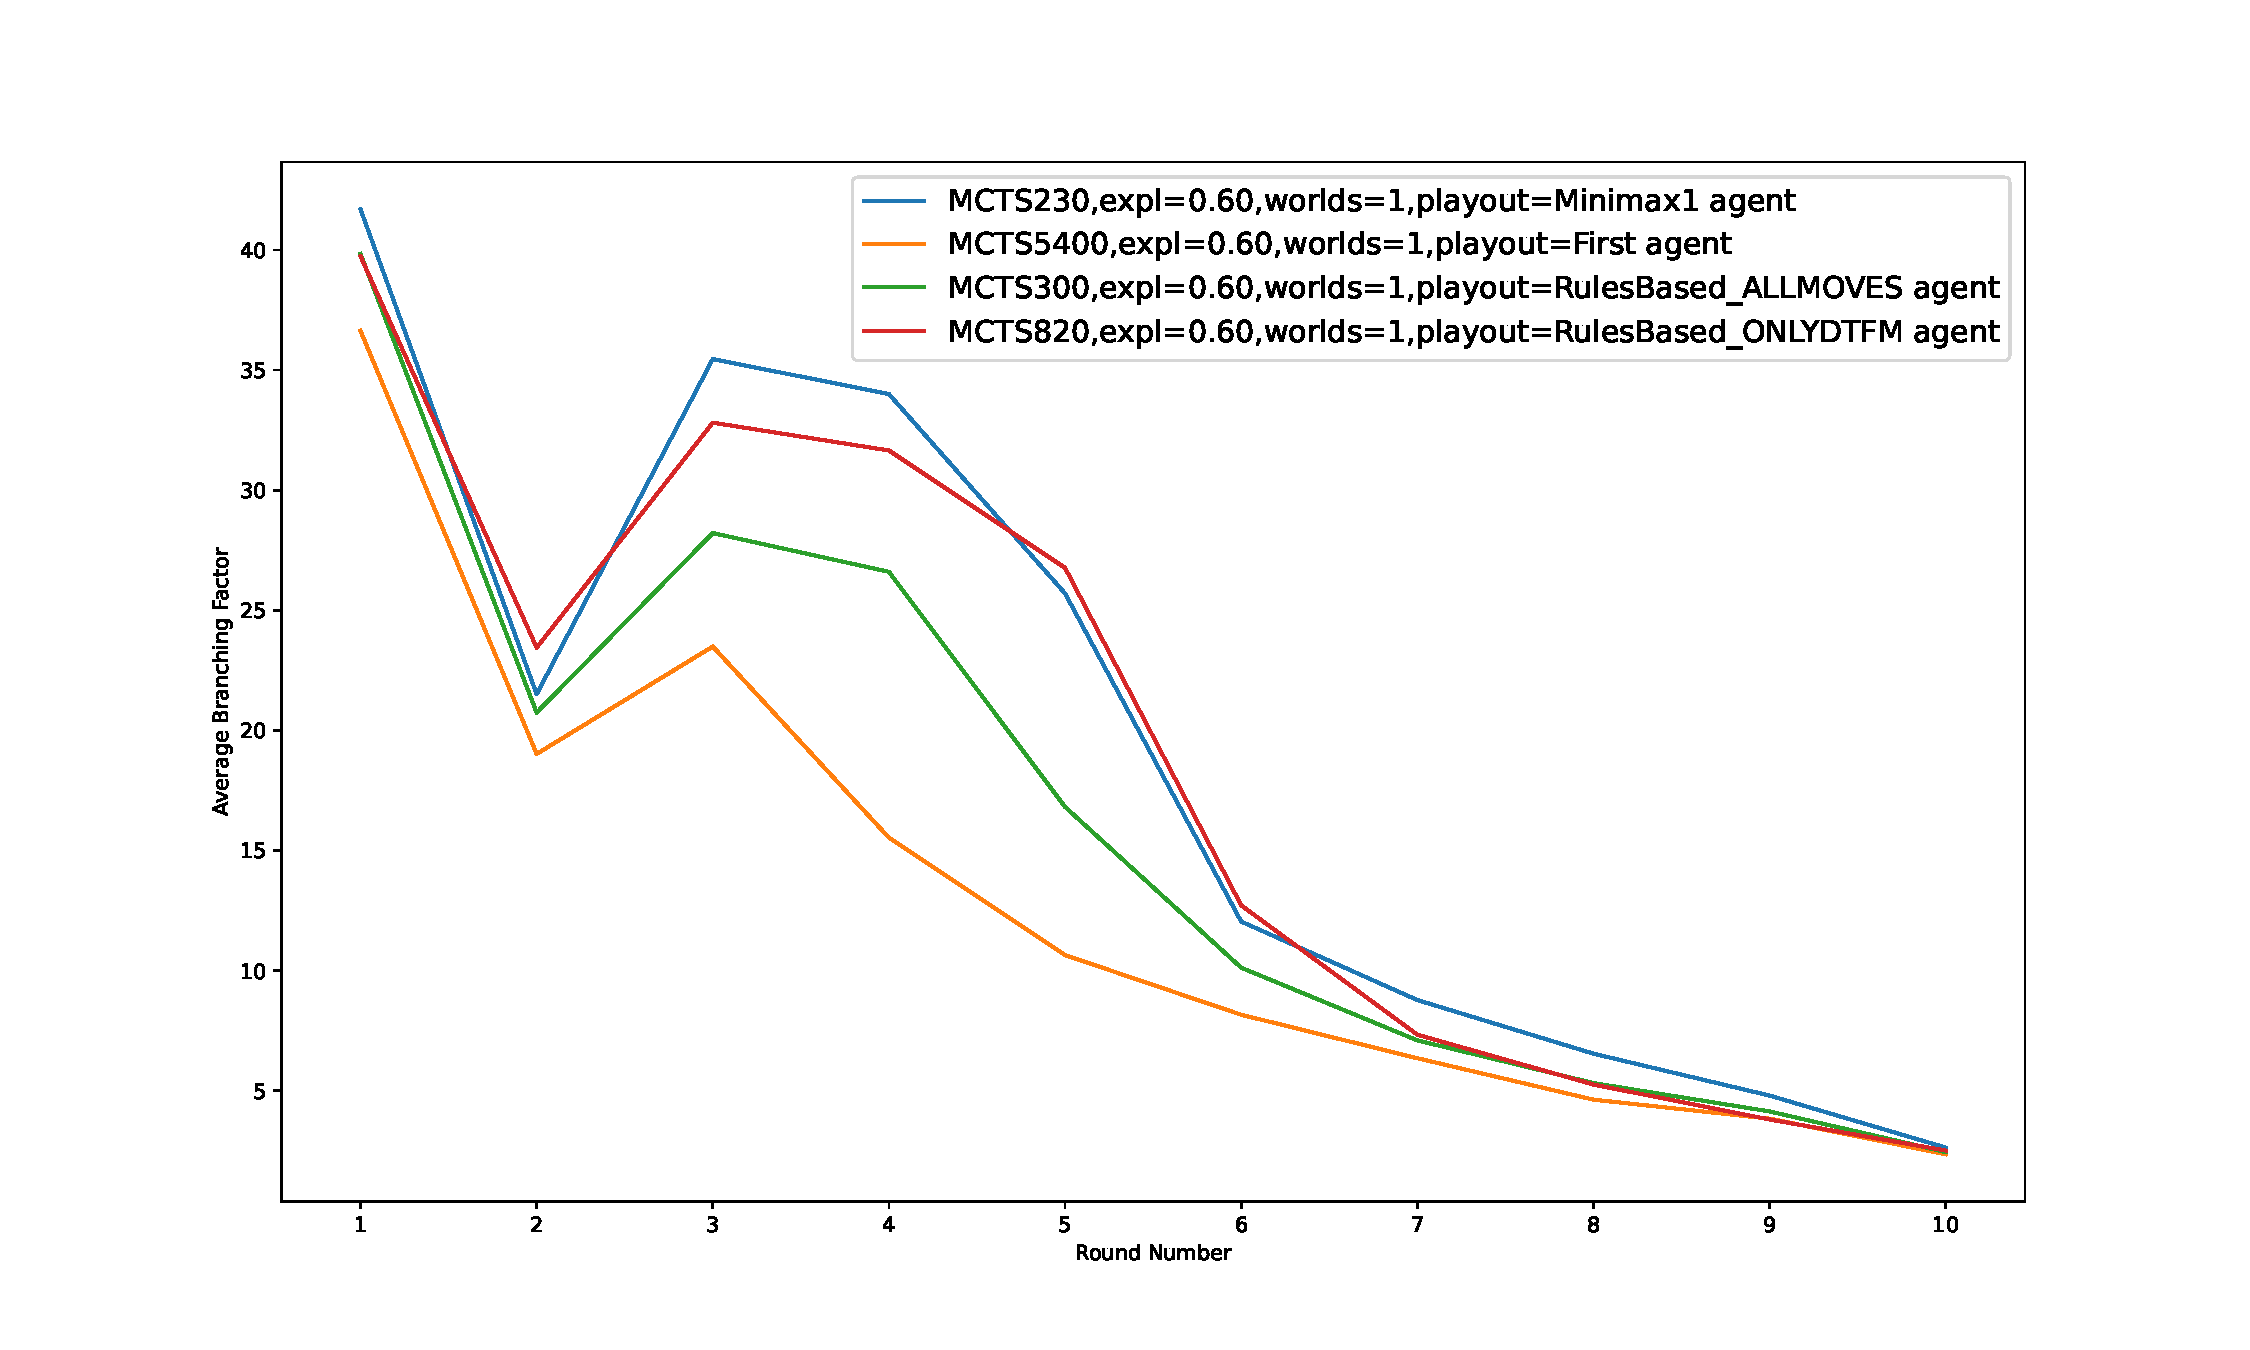
\includegraphics[width=180mm]{img/mcts_average_branching_factor.pdf}}}
    \label{fig:example}
\end{figure}

The figure shows that the average branching factor for the MCTS agents is the highest in round 1 with a value slightly above 40. So the algorithm's selection
strategy could make a higher difference, I choose to configure a minimum of 80 iteration count for the agents. 


As already mentioned in Section \ref{subsec:MCTS_Selection_UCT}, an often chosen value for the exploration constant is $\sqrt{2}$. I chose to experiment with 
values $[0.6, 0.8, 1.0, 1.2, 1.4, 1.6, 1.8, 2.0]$. I ran separate experiments for the four playout strategies. The following figures illustrate the highest
win count in every iteration count-determinizing world count division displaying the exploration constant used. Each tournament contained 100 games and every
exploration constant, iteration count-determinizing world count pair has a corresponding tournament. The results can be found in the \texttt{tournament\_results/mcts\_playout\_first\_exploration},
\texttt{tournament\_results/mcts\_playout\_minimax1\_exploration}, \\ \texttt{tournament\_results/mcts\_playout\_rules\_based\_only\_dtfm\_exploration} and the 
\texttt{tournament\_results/mcts\_playout\_rules\_based\_all\_moves\_exploration} directories. All the tournaments were run against the Minimax agent with search depth of 3
and determinizing world count of 1.

\begin{figure}[H]
    \caption{Exploration constants producing the highest win rate in different iteration count-determinizing world count divisions for the First playout}
    \centerline{\mbox{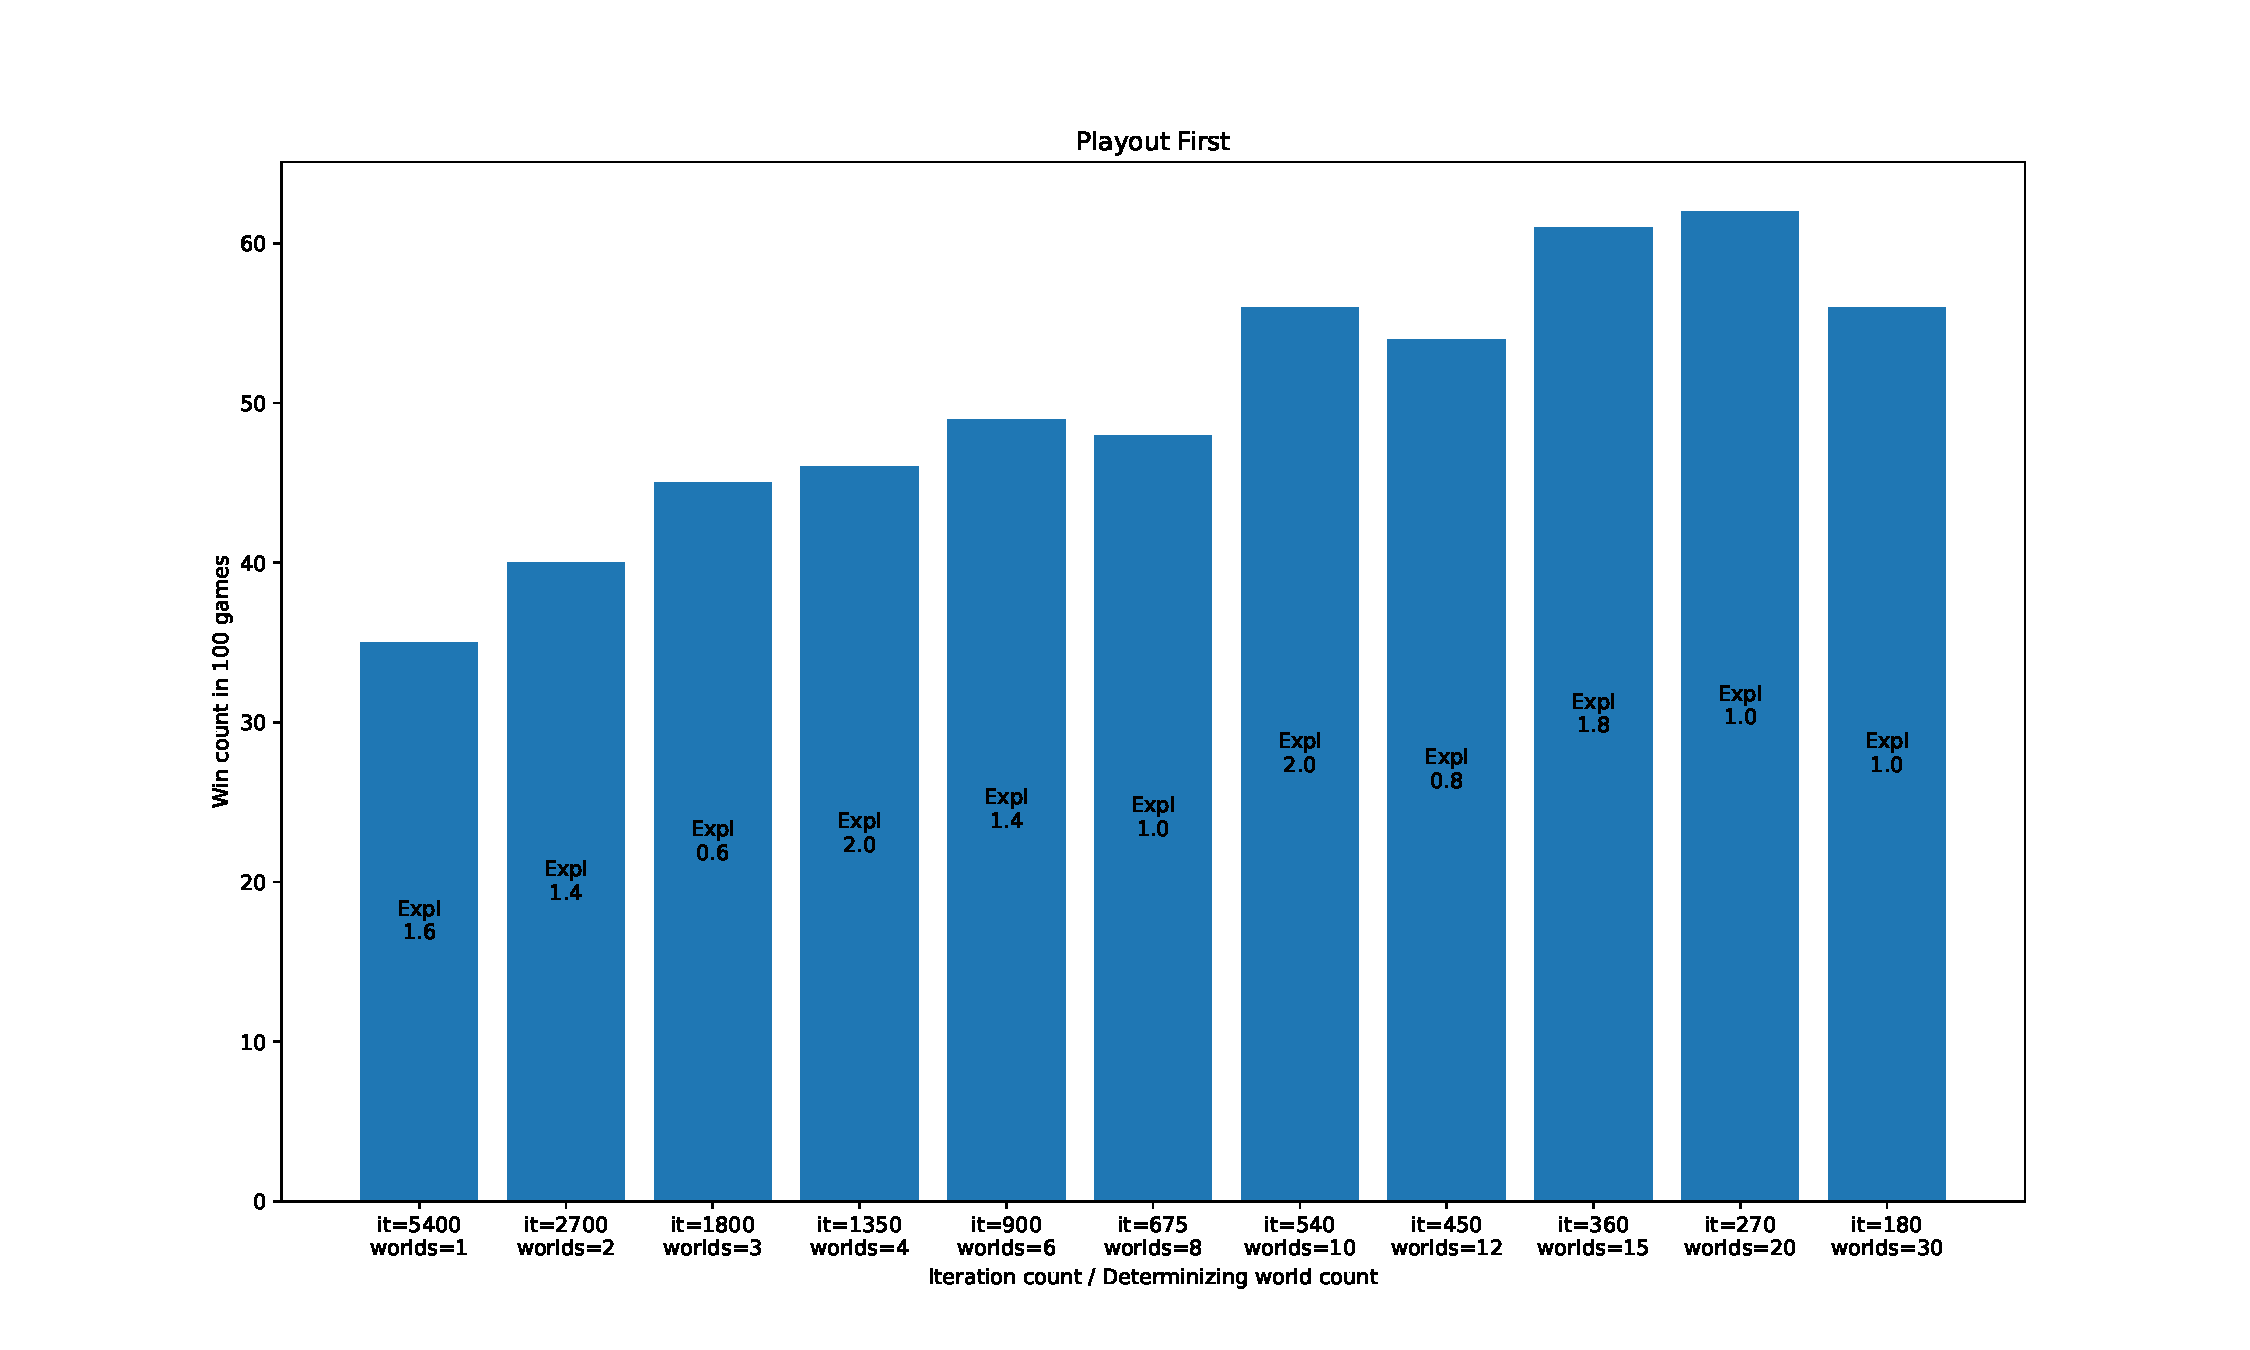
\includegraphics[width=180mm]{img/mcts_expl_worldcount_First.pdf}}}
    \label{fig:example}
\end{figure}

\begin{figure}[H]
    \caption{Exploration constants producing the highest win rate in different iteration count-determinizing world count divisions for the Minimax playout}
    \centerline{\mbox{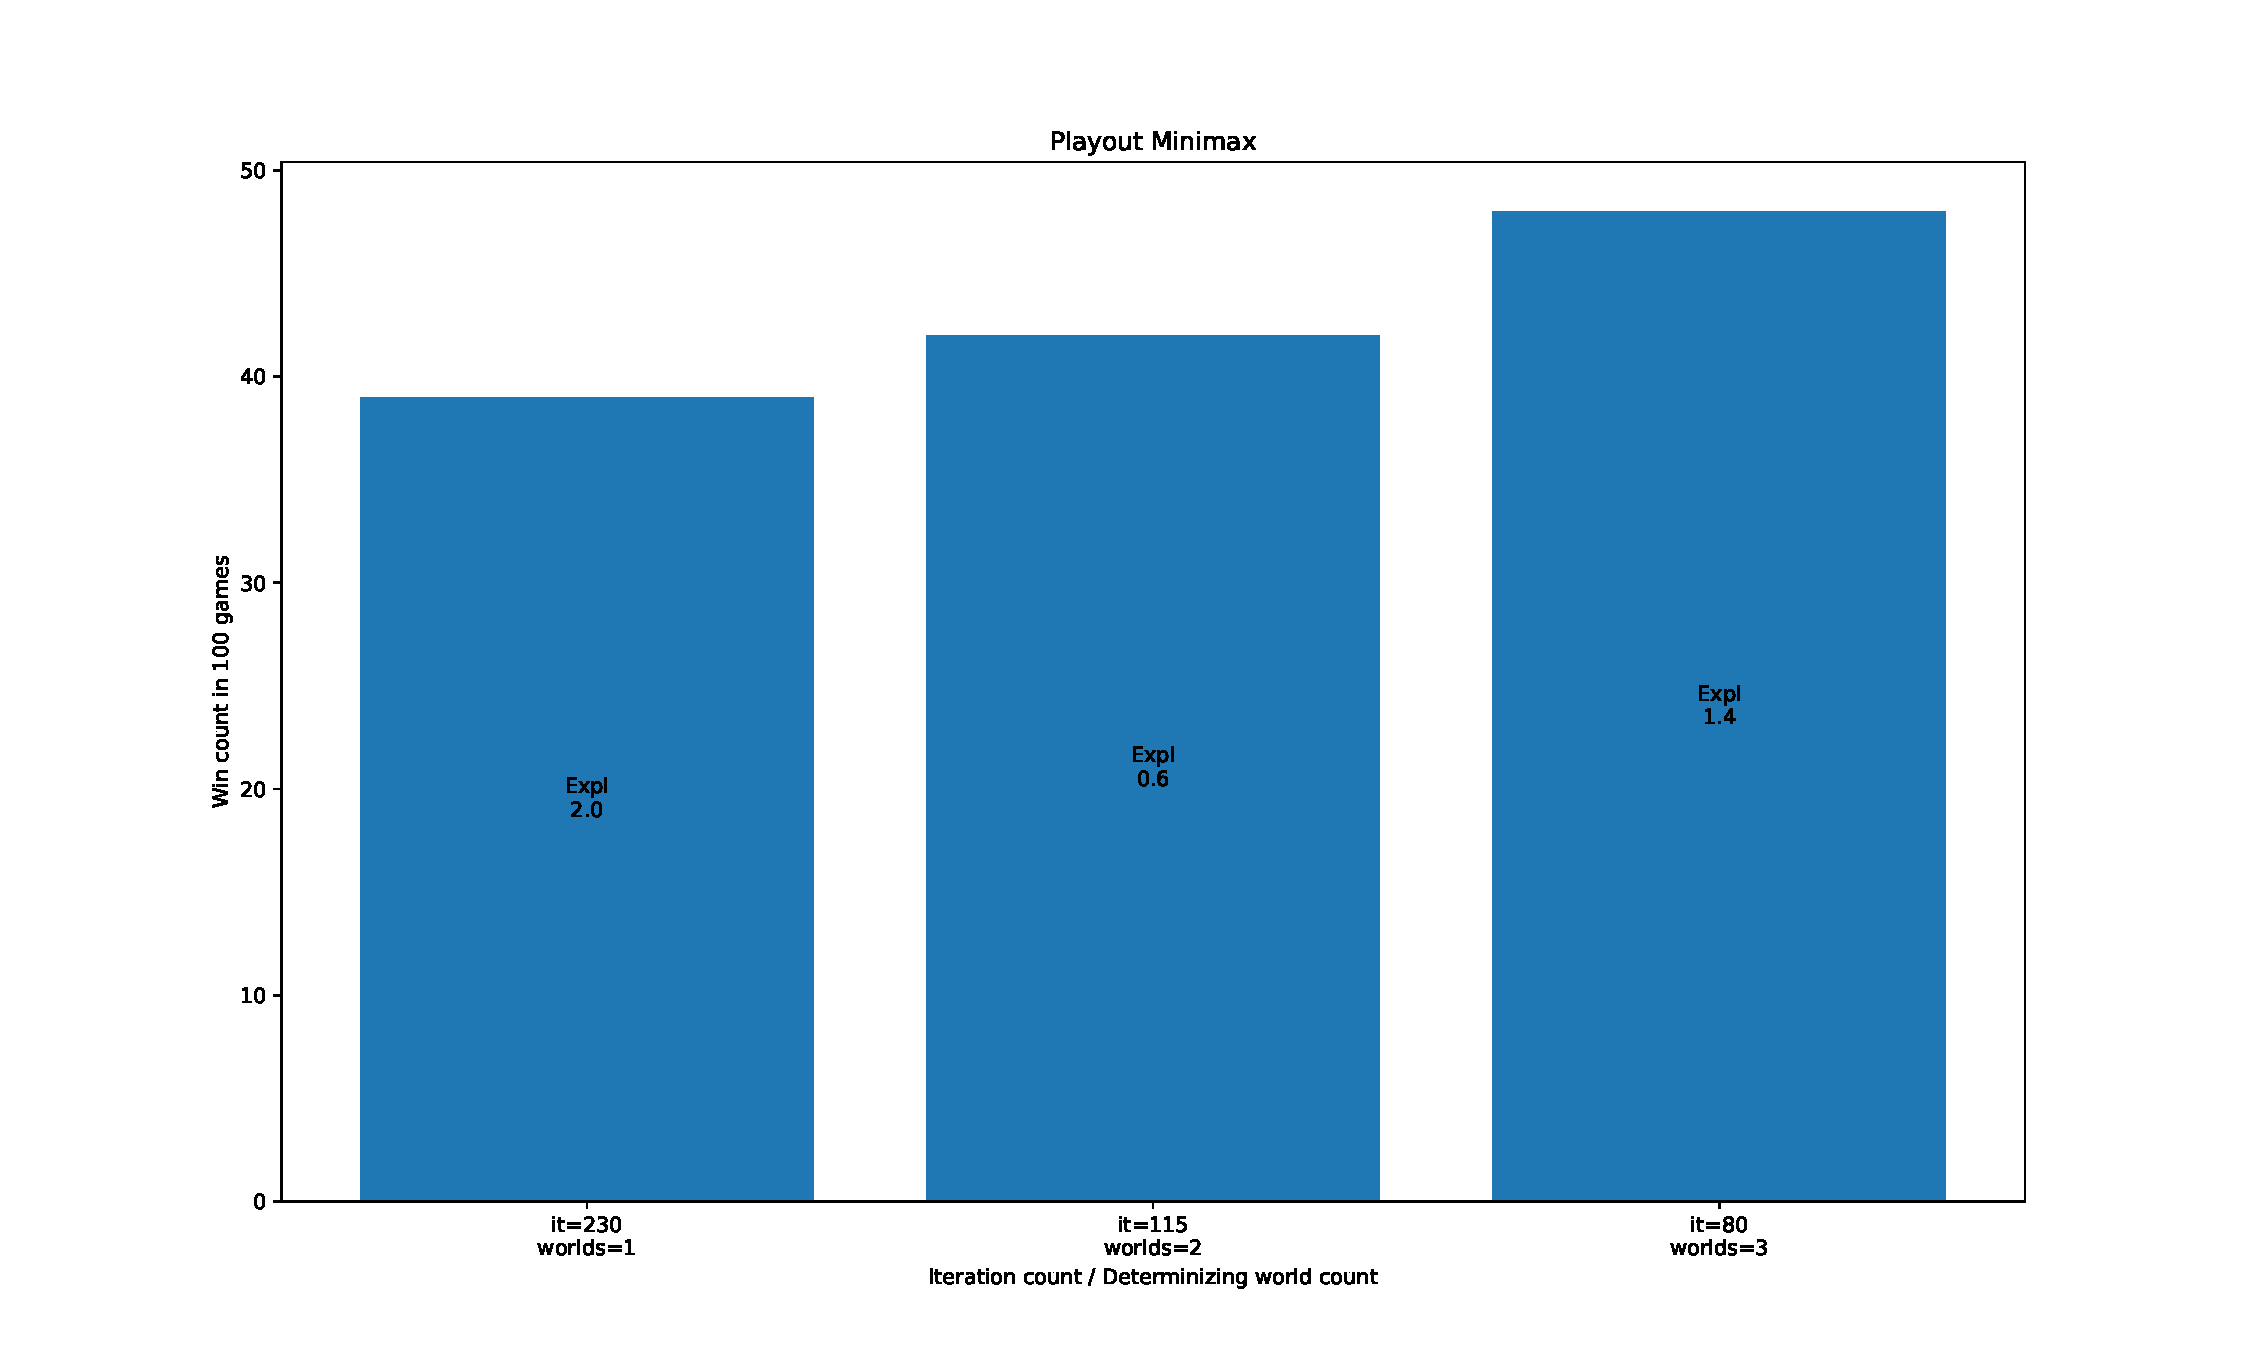
\includegraphics[width=170mm]{img/mcts_expl_worldcount_Minimax.pdf}}}
    \label{fig:example}
\end{figure}


\begin{figure}[H]
    \caption{Exploration constants producing the highest win rate in different iteration count-determinizing world count divisions for the Rules-based ALL MOVES playout}
    \centerline{\mbox{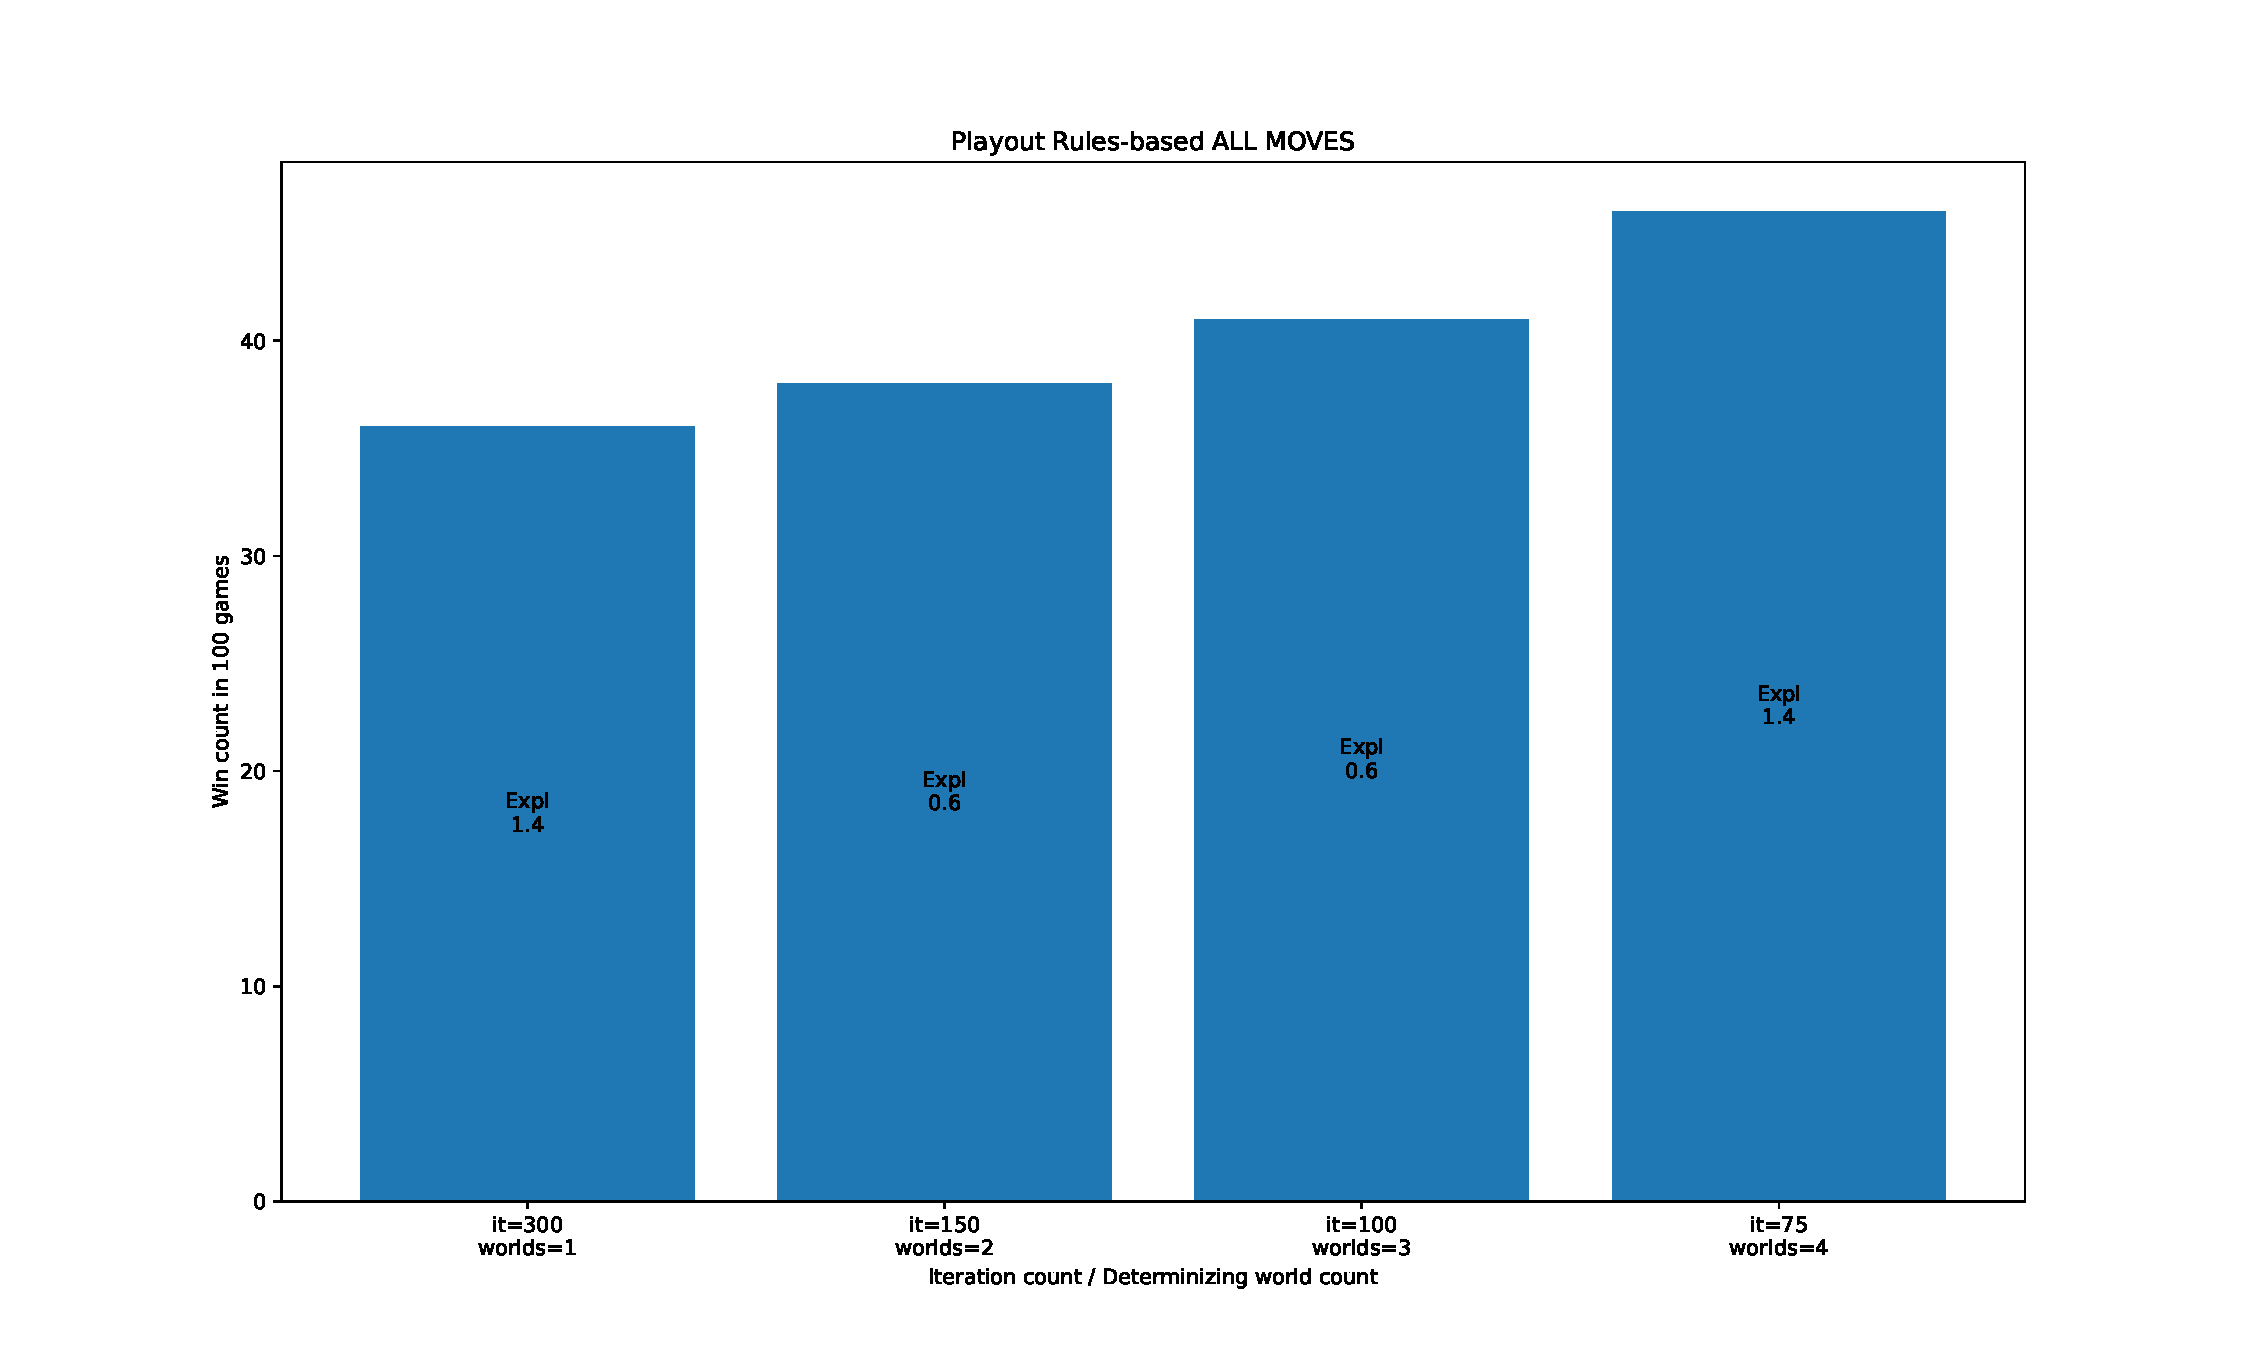
\includegraphics[width=170mm]{img/mcts_expl_worldcount_Rules-based ALL MOVES.pdf}}}
    \label{fig:example}
\end{figure}

\begin{figure}[H]
    \caption{Exploration constants producing the highest win rate in different iteration count-determinizing world count divisions for the Rules-based ONLY DTFM playout}
    \centerline{\mbox{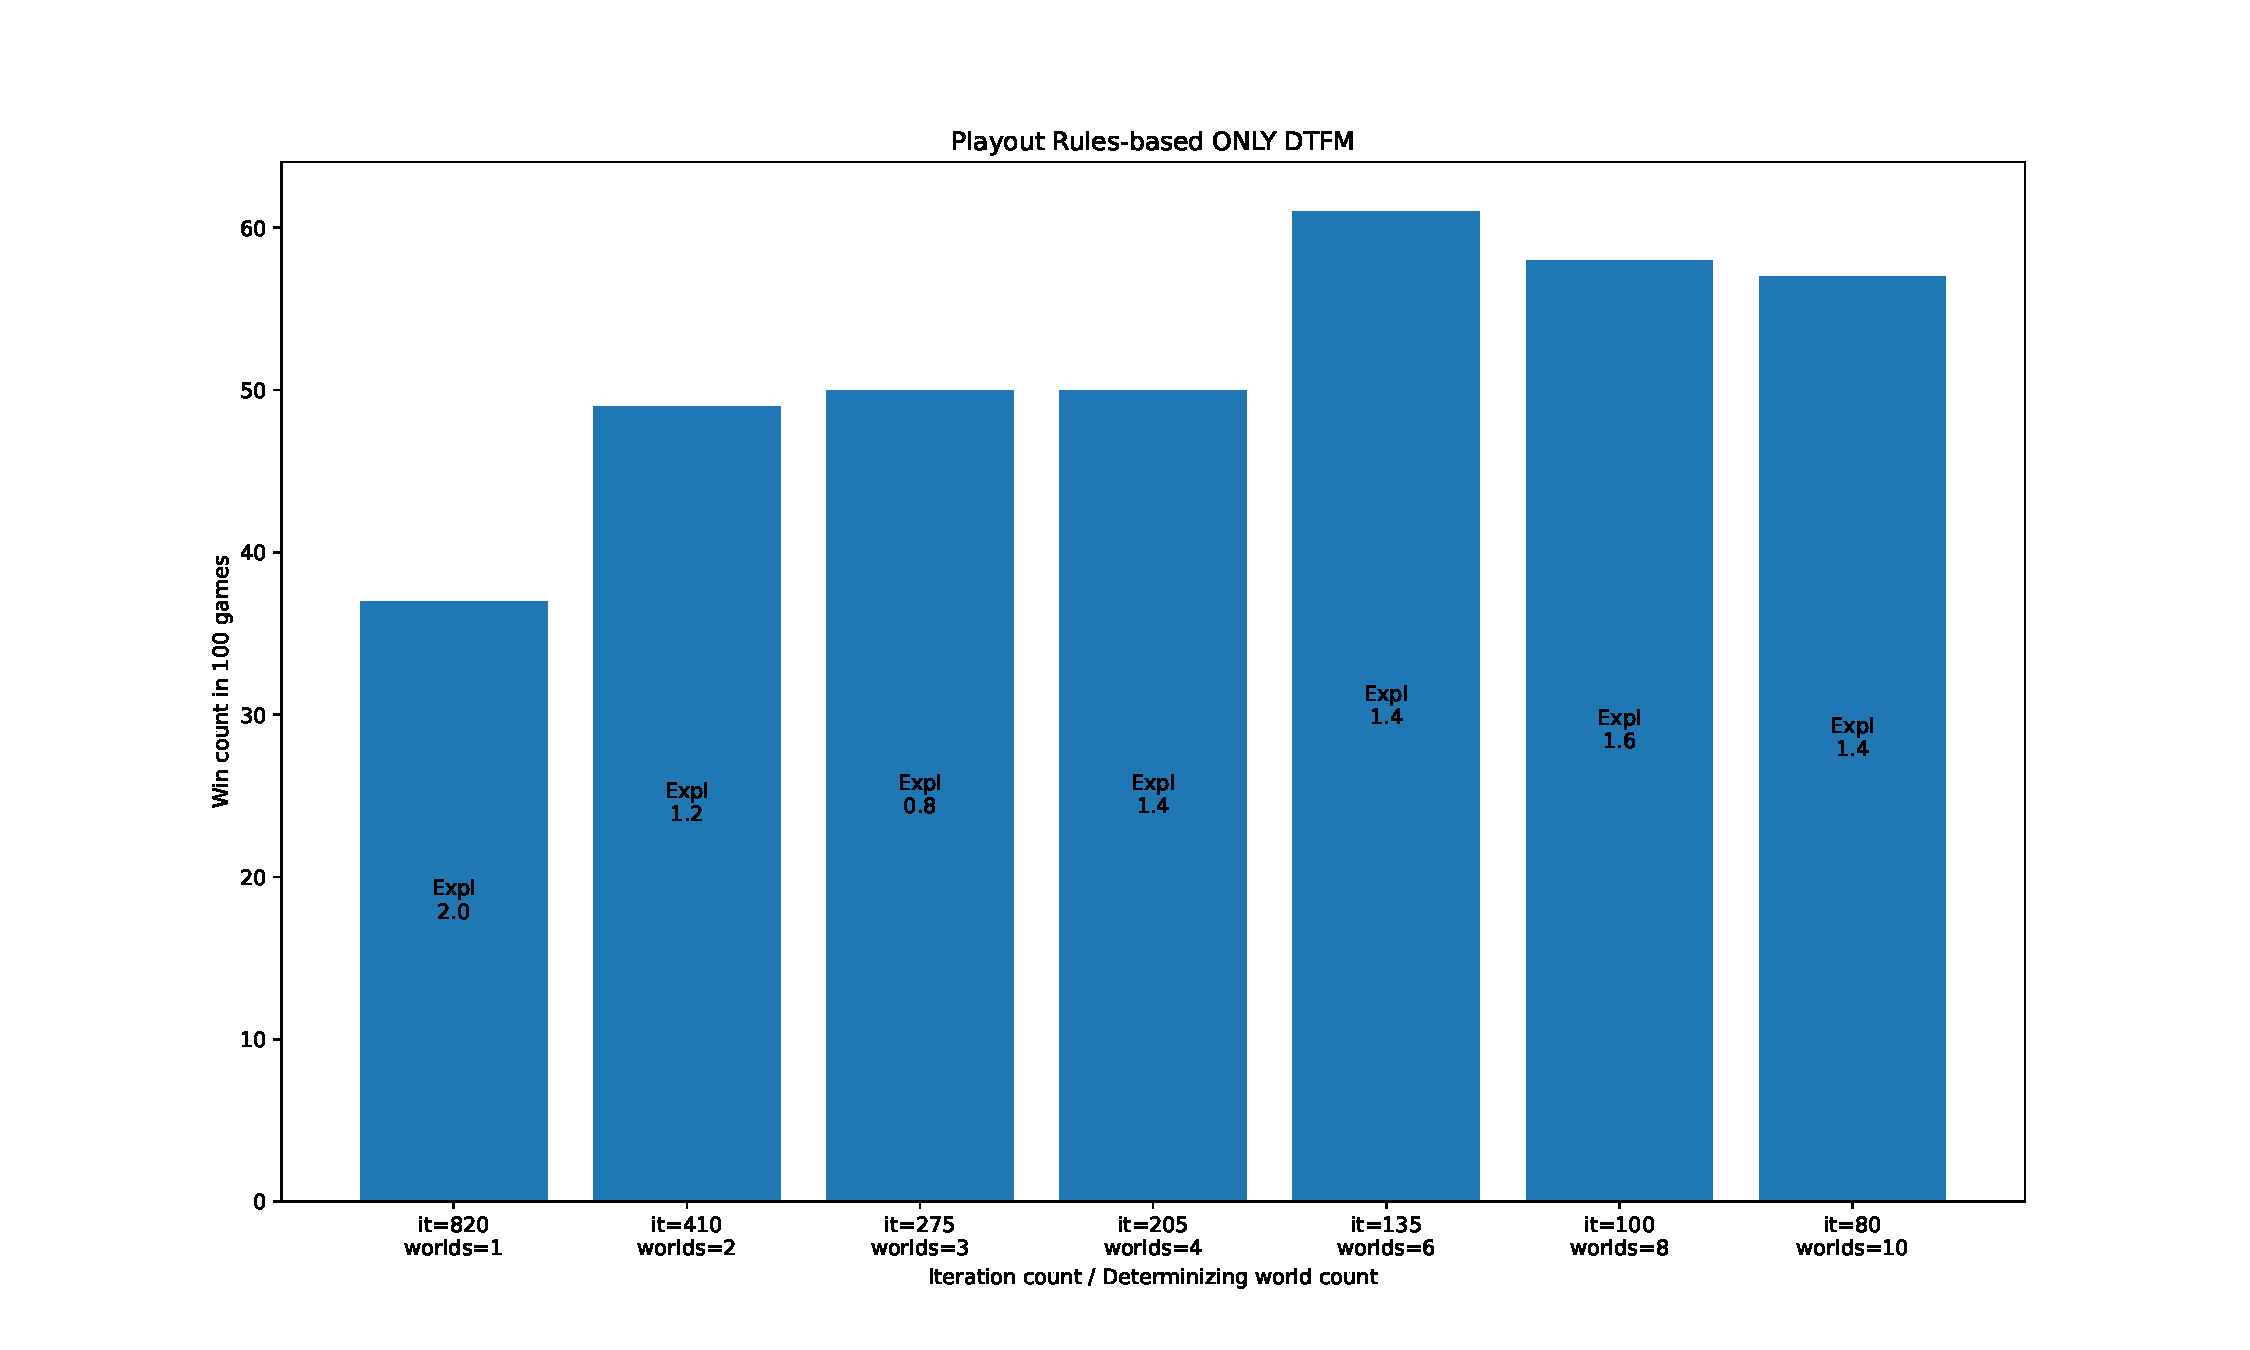
\includegraphics[width=180mm]{img/mcts_expl_worldcount_Rules-based ONLY DTFM.pdf}}}
    \label{fig:example}
\end{figure}

As seen in the second and third figures, the Minimax and the Rules-based ALL MOVES playout strategies don't achieve even 50\% of wins with any of the configured
exploration constants. For this reason, in the upcoming experiments, I will use following the configurations:


\begin{table}[H] 
    \centering
    \begin{tabular}{|c|c|c|} 
        \hline
        \textbf{Playout strategy} & \textbf{Iteration count} & \textbf{Exploration constant} \\ \hline
        First & 270 & 1.0 \\ \hline
        First & 360 & 1.8 \\ \hline
        Rules-based only dtfm & 135 & 1.4 \\ \hline
    \end{tabular}
    \caption{Strongest MCTS configurations against the Minimax-depth=3,worlds=1 agent}
    %\label{tab:example_table}
\end{table}


\section{Minimax}


\subsection{Hyperparameters} \label{subsec:Minimax_Hyperparameters}

Choosing the constants that represent the weights of the component weights in the HeuristicConstants structure is not a trivial task. After trying out different 
constants manually, I decided to automatize this task by creating random configurations, running some tournaments and evaluating the results. The two main attributes 
that could be maximized during this experiment are average points and win count. I chose to maximize average points because the experiment is run between
a minimax agent and one configured agent but the goal is to have the agent as strong as possible against all the other agents so choosing 
a configuration based on the win count against a concrete agent is the weaker option.


To obtain the current configuration, I ran an experiment of 10000 tournaments between the rules-based player and the minimax player. 
I chose to select the top 30 results i.e. the 30 tournaments that produced the highest average score for the minimax player. To achieve
this, I ran the following commands:

\begin{verbatim}
$ ./tournaments/minimax_random_config_experiment.py -v -e 10000  \ 
    -o heuristic_constant_experiments -p rules-based-strategy=only_dtfm 
$ ./tournaments/heuristic_const_experiment_evaluator.py -top 30 \
    -i tournament_results/heuristic_constant_experiments/ 
\end{verbatim}


and chose the configuration with the highest average score. This experiment produced the following weight constants:
\begin{table}[H] 
    \centering
    \begin{tabular}{|c|c|} % two centered columns
    \hline
    Weight constant name & Weight constant value \\ \hline
    OpponentInfluencingFactor & 9.83724229656198    \\ \hline
    PuocCompletablePower & 3.1133889400588606 \\ \hline
    MinusPointsPerUncompletableField & 373 \\ \hline
    CompletedPointsWeight & 416    \\ \hline
    MinusPointsPerUncompletablePuocPoints & 7  \\ \hline
    \end{tabular}
    \caption{Currently used heuristic weight constants}
    \label{tab:example_table}
\end{table}

Please notice that running this experiment with the current build will produce a different outcome since when I ran this experiment, I was using a previous build
and the old configuration for the minimax agent. The results of this experiment can be found in the \texttt{tournament\_results/heuristic\_constant\_experiments} directory.


\subsection{Search Depth and Determinizing World Count}

There are two other configurable parameters left after choosing the globally used heuristic weight constants as described in the previous section.
The goal of this section is to find the perfect balance between search depth and determinizing world count producing the strongest possible configuration.

The following table illustrates the determinizing world count for search depths fitting the time limit:

\begin{table}[H] 
    \centering
    \begin{tabular}{|c|c|}
        \hline 
        \textbf{Search depth} & \textbf{Determinizing world count} \\ \hline
        1 & 2000 \\ \hline
        2 & 200 \\ \hline
        3 & 20 \\ \hline
        4 & 2 \\ \hline
    \end{tabular}
    \caption{Minimax configurations fitting the time limit}
\end{table}




\section{Final Results}

In this section, I will present the final results of the players. This experiment employs a round-robin format meaning that every player plays against every other player.
First, a fixed number of 320 games were run in each tournament. To achieve the best results possible, additional tournaments of 160 games were run until a confidence interval
of 50\% was reached for any of the players. The upper bound for the number of games played between two concrete AI players was set to 2240. 
To eliminate any type of advantage, the tournaments were run with \texttt{the -b option} specified meaning that each seed is used twice, once with player1 as the initial player, 
and once with player2 as the initial player. This method helps to avoid any advantage connected with being the initial or the subsequent player. 

The following tables display the confidence interval and total games played between all other players and the minimax agents. Both tables have on the field in the i-th row
and j-th column the confidence interval of the j-th column's agent against the i-th row's agent. The following abbreviations for agent names are used in the following tables:
\begin{description}
    \item[Mini1,2000] - minimax-depth=1,worlds=2000
    \item[Mini2,200] - minimax-depth=2,worlds=200
    \item[Mini3,20] - minimax-depth=3,worlds=20
    \item[Mini4,2] - minimax-depth=4,worlds=2
    \item[MCTS135\_OD] - mcts-it=135,expl=1.4,worlds=6,playout=rules-based-strategy=only\_dtfm
    \item[MCTS270\_First] - mcts-it=270,expl=1.0,worlds=20,playout=first
    \item[MCTS360\_First] - mcts-it=360,expl=1.8,worlds=15,playout=first
    \item[RB\_OD] - rules-based-strategy=only\_dtfm
    \item[RB\_AM] - rules-based-strategy=all\_moves
\end{description}

\renewcommand{\arraystretch}{0.7} % Adjust the spacing between rows

\begin{table}[H] 
    \centering
    \begin{tabular}{|c|c|c|c|c|} 
        %\textbf{Search depth} & \textbf{Determinizing world count} \\ 
        \hline
        \text{ } & \textbf{Mini1,2000} & \textbf{Mini2,200} & \textbf{Mini3,20} & \textbf{Mini4,2} \\ \hline

        \multirow{2}{*}{\textbf{Mini1,2000}} & & 320 & 480 & 2240 \\
        & & 50.7\%-63.5\% & 52.0\%-62.4\% & 48.8\%-53.7\% \\ \hline
        \multirow{2}{*}{\textbf{Mini2,200}} & 320 & & 2240 & 2240 \\
        & 36.5\%-49.3\% & & 48.3\%-53.3\% & 47.5\%-52.5\% \\ \hline
        \multirow{2}{*}{\textbf{Mini3,20}} & 480 & 2240 & & 2240 \\
        & 37.6\%-48.0\% & 46.7\%-51.7\% & & 45.5\%-50.4\% \\ \hline
       \multirow{2}{*}{\textbf{Mini4,2}} & 2240 & 2240 & 2240 & \\
        & 46.3\%-51.2\% & 47.5\%-52.5\% & 49.6\%-54.5\% & \\ \hline

       \multirow{2}{*}{\textbf{MCTS135\_OD}} & 2240 & 2240 & 1280 & 1440 \\
        & 46.9\%-51.8\% & 48.7\%-53.6\% & 50.0\%-56.5\% & 50.3\%-56.4\% \\ \hline

       \multirow{2}{*}{\textbf{MCTS270\_First}} & 320 & 320 & 320 & 320 \\
        & 51.0\%-63.8\% & 51.0\%-63.8\% & 58.0\%-70.3\% & 58.6\%-70.9\% \\ \hline
       \multirow{2}{*}{\textbf{MCTS360\_First}} & 512 & 320 & 320 & 320 \\
        & 50.7\%-60.9\% & 55.7\%-68.2\% & 54.5\%-67.1\% & 56.0\%-68.5\% \\ \hline
       \multirow{2}{*}{\textbf{RB\_OD}} & 320 & 320 & 320 & 320 \\
        & 53.8\%-66.5\% & 60.8\%-73.0\% & 57.6\%-70.0\% & 57.0\%-69.4\% \\ \hline
       \multirow{2}{*}{\textbf{RB\_AM}} & 320 & 320 & 320 & 320 \\
        & 58.0\%-70.3\% & 63.7\%-75.6\% & 67.7\%-79.0\% & 62.5\%-74.4\% \\ \hline
       \multirow{2}{*}{\textbf{First}} & 320 & 320 & 320 & 320 \\
        & 94.5\%-98.9\% & 96.8\%-99.7\% & 93.7\%-98.5\% & 95.8\%-99.4\% \\ \hline
       \multirow{2}{*}{\textbf{Random}} & 320 & 320 & 320 & 320 \\
        & 97.2\%-99.9\% & 97.8\%-100.0\% & 97.2\%-99.9\% & 97.8\%-100.0\% \\ \hline
        
    \end{tabular}
    \caption{Minimax confidence intervals against all the other agents}
\end{table}

Looking at the last 4 rows of this table, it is clear that all the minimax agents easily won the tournaments against the First, Random
and the two strategies of the Rules-based agents. All these tournaments ended after the minimum amount of games were played that this experiment defines.
Deciding which minimax configuration is the strongest is not straightforward. The first 4 rows indicate that the 6 tournaments run between
the minimax agents against each other, 4 of the tournaments continued to the maximum number of games chosen for this experiment. The MCTS agents
with the First playout strategy produced weak results against all the minimax configurations. The single strong opponent was the MCTS agent
with the Rules-based only dtfm playouts. According to this experiment, the two strongest configurations were the one with a search depth of 3
and the one with the search depth of 4.

\begin{table}[H] 
    \centering
    \begin{tabular}{|c|c|c|c|} 
        %\textbf{Search depth} & \textbf{Determinizing world count} \\ 
        \hline
        \text{ } & \textbf{MCTS270\_First} & \textbf{MCTS360\_First} & \textbf{MCTS135\_OD} \\ \hline
        \multirow{2}{*}{\textbf{MCTS270\_First}} & & 2240 & 2240 \\
        & & 45.9\%-50.9\% & 48.1\%-53.0\% \\ \hline
        \multirow{2}{*}{\textbf{MCTS360\_First}} & 2240 & & 2240 \\
        & 49.1\%-54.1\% & & 48.2\%-53.1\% \\ \hline
        \multirow{2}{*}{\textbf{MCTS135\_OD}} & 2240 & 2240 & \\
        & 47.0\%-51.9\% & 46.9\%-51.8\% & \\ \hline
        \multirow{2}{*}{\textbf{Mini3,20}} & 320 & 320 & 1280 \\
        & 29.7\%-42.0\% & 32.9\%-45.5\% & 43.5\%-50.0\% \\ \hline
        \multirow{2}{*}{\textbf{Mini4,2}} & 320 & 320 & 1440 \\
        & 29.1\%-41.4\% & 31.5\%-44.0\% & 43.6\%-49.7\% \\ \hline
        \multirow{2}{*}{\textbf{Mini2,200}} & 320 & 320 & 2240 \\
        & 36.2\%-49.0\% & 31.8\%-44.3\% & 46.4\%-51.3\% \\ \hline
        \multirow{2}{*}{\textbf{Mini1,2000}} & 320 & 512 & 2240 \\
        & 36.2\%-49.0\% & 39.1\%-49.3\% & 48.2\%-53.1\% \\ \hline
        \multirow{2}{*}{\textbf{RB\_OD}} & 1280 & 1600 & 320 \\
        & 50.9\%-57.4\% & 50.5\%-56.3\% & 52.6\%-65.3\% \\ \hline
        \multirow{2}{*}{\textbf{RB\_AM}} & 320 & 480 & 320 \\
        & 55.1\%-67.6\% & 51.6\%-62.0\% & 62.5\%-74.4\% \\ \hline
        \multirow{2}{*}{\textbf{First}} & 320 & 320 & 320 \\
        & 92.9\%-98.0\% & 95.4\%-99.2\% & 96.8\%-99.7\% \\ \hline
        \multirow{2}{*}{\textbf{Random}} & 320 & 320 & 320 \\
        & 95.8\%-99.4\% & 96.3\%-99.6\% & 97.8\%-100.0\% \\ \hline
    
    \end{tabular}
    \caption{MCTS confidence intervals against all the other agents}
\end{table}

The last four rows show similar results as in the case of the minimax player meaning that the MCTS player is stronger than the 
First, Random and Rules-based agents. From the results of the tournaments run between the MCTS players, it is not possible
to choose the strongest configuration. Lastly, looking at the results against the minimax agent, the clear winner of the MCTS
configurations is the MCTS135\_OD.

\section{Deterministic vs Non-Deterministic World Results}

In this section, I will compare the results presented in the previous section with the same tournaments run in the deterministic world.
The same type of agents in the non-deterministic world are compared with the agents having the same computational resources in the 
deterministic world. This means that the minimax agent will use the same search depth and the MCTS player will use the same amount of iterations.

The main idea is to compare how imperfect information affects the different players. For this reason, I am comparing the following agents:

\begin{description}
    \item[minimax-depth=4]
    \item[mcts-it=820,expl=1.4,playout=rules-based-strategy=only\_dtfm]
    \item[mcts-it=5400,expl=1.0,playout=first]
    \item[mcts-it=5400,expl=1.8,playout=first]
\end{description}

Every tournament contained 320 games and the following table illustrates the results:

\begin{table}[H] 
    \centering
    \begin{tabular}{|c|c|c|c|c|} 
        \hline
        \textbf{Player name} & \textbf{Tournament wins} & \textbf{Confidence interval} \\ \hline
        MCTS820,expl=1.4,playout=only\_dtfm & 3 & 61.1\%-68.3\% \\ \hline
        Minimax4 & 2 & 45.9\%-53.4\% \\ \hline
        MCTS5400,expl=1.0,playout=first & 1 & 41.4\%-48.9\% \\ \hline
        MCTS5400,expl=1.4,playout=first & 0 & 36.8\%-44.1\% \\ \hline
    
    \end{tabular}
    \caption{Deterministic world results}
\end{table}

The MCTS player with the only\_dtfm playout strategy is clearly the strongest player in the deterministic world.

\chapter*{Conclusion}
\addcontentsline{toc}{chapter}{Conclusion}


%%% Bibliography
%%% Bibliography (literature used as a source)
%%%
%%% We employ biblatex to construct the bibliography. It processes
%%% citations in the text (e.g., the \cite{...} macro) and looks up
%%% relevant entries in the bibliography.bib file.
%%%
%%% See also biblatex settings in thesis.tex.

%%% Generate the bibliography. Beware that if you cited no works,
%%% the empty list will be omitted completely.

% We let bibliography items stick out of the right margin a little
\def\bibfont{\hfuzz=2pt}

\printbibliography[heading=bibintoc]

%%% If case you prefer to write the bibliography manually (without biblatex),
%%% you can use the following. Please follow the ISO 690 standard and
%%% citation conventions of your field of research.

% \begin{thebibliography}{99}
%
% \bibitem{lamport94}
%   {\sc Lamport,} Leslie.
%   \emph{\LaTeX: A Document Preparation System}.
%   2nd edition.
%   Massachusetts: Addison Wesley, 1994.
%   ISBN 0-201-52983-1.
%
% \end{thebibliography}


%%% Figures used in the thesis (consider if this is needed)
\listoffigures

%%% Tables used in the thesis (consider if this is needed)
%%% In mathematical theses, it could be better to move the list of tables to the beginning of the thesis.
\listoftables

%%% Abbreviations used in the thesis, if any, including their explanation
%%% In mathematical theses, it could be better to move the list of abbreviations to the beginning of the thesis.
\chapwithtoc{List of Abbreviations}
\begin{acronym}
	\acro{GUI}{Graphical user interface}
	\acro{CLI}{Command-line interface}
	\acro{DTFM}{Die-to-field moves - moves that place a die onto a field}
	\acro{PrOC}{Private Objective Card}
	\acro{PuOC}{Public Objective Card}
	\acro{TC}{Tool Card}
\end{acronym}

%%% Attachments to the thesis, if any. Each attachment must be referred to
%%% at least once from the text of the thesis. Attachments are numbered.
%%%
%%% The printed version should preferably contain attachments, which can be
%%% read (additional tables and charts, supplementary text, examples of
%%% program output, etc.). The electronic version is more suited for attachments
%%% which will likely be used in an electronic form rather than read (program
%%% source code, data files, interactive charts, etc.). Electronic attachments
%%% should be uploaded to SIS. Allowed file formats are specified in provision
%%% of the rector no. 72/2017. Exceptions can be approved by faculty's coordinator.
\appendix
\chapter{Attachments}

\section{First Attachment}

\end{document}
